% !TeX program = xelatex
\documentclass[acmsmall,screen,review,anonymous]{acmart}

\setcopyright{none}
\copyrightyear{2027}
\acmYear{2027}
\acmDOI{}
\acmConference[FSE 2027]
  {The ACM International Conference on the Foundations of Software Engineering}
  {July 12--16, 2027}
  {Shenzhen, China}
\acmISBN{}
% acmsmall conference mode: match upstream acmConference header/footer selection.
% Compatibility for installed acmart 2.19; no journal volume/article is assigned.
\makeatletter
\@ACM@journal@bibstrip@or@togfalse
\makeatother
\settopmatter{printfolios=true}

\usepackage[ruled,vlined,linesnumbered]{algorithm2e}
\usepackage{array}
\usepackage{placeins}
\usepackage{needspace}
\usepackage{xurl}
\usepackage{xr-hyper}
\externaldocument[][nocite]{build/technical_appendix}[technical_appendix.pdf]
\usepackage{tikz}
\usetikzlibrary{automata,positioning,arrows.meta}
\usepgflibrary{fpu}
\vbadness=10000

\usepackage{iftex}
\ifXeTeX\else
  \PackageError{main}{This manuscript requires XeLaTeX}%
    {Select XeLaTeX as the compiler, or keep the supplied latexmkrc file.}
\fi
\AtBeginDocument{%
  \providecommand\BibTeX{{Bib\TeX}}}

\newcommand{\Post}{\mathsf{Post}}
\newcommand{\Safe}{\mathsf{Safe}}
\newcommand{\Goal}{Q_{\mathrm{goal}}}
\newcommand{\rank}{\mathsf{rk}}
\newcommand{\ActT}{\mathsf{ActiveM}}
\newcommand{\Init}{\mathsf{Init}}
\newcommand{\Reach}{\mathsf{Reach}}
\newcommand{\SuccSet}{\mathsf{Succ}}
\newcommand{\En}{\mathsf{En}}
\newcommand{\Cand}{\mathsf{Next}}
\newcommand{\Sigmauc}{\Sigma_{\mathrm{uc}}}
\newcommand{\Sigmac}{\Sigma_{\mathrm{c}}}
\newcommand{\SigmaN}{\Sigma_{\mathrm{N}}}
\newcommand{\SigmaU}{\Sigma_{\mathrm{upd}}}
\newcommand{\CLnew}{\mathsf{CL}^{\mathrm{new}}}
\newcommand{\ustart}[1]{\mathsf{start}(#1)}
\newcommand{\ustop}[1]{\mathsf{stop}(#1)}

% Derived from validated returned raw; elapsed/RSS are single-trial references, not medians.
\providecommand{\ADDirectFullWins}{14}
\providecommand{\ADDirectFullTimeouts}{13}
\providecommand{\ADWorkflowCapSeconds}{1200}
\providecommand{\ADWorkflowElapsedSeconds}{1201.7}
\providecommand{\ADWorkflowPeakRSSGiB}{13.9}
\providecommand{\ADPCCapSeconds}{3600}
\providecommand{\ADPCElapsedSeconds}{3605.2}
\providecommand{\ADPCPeakRSSGiB}{67.1}

% Generated from validated Xeon raw; do not edit.
\newcommand{\LFConditions}{21}
\newcommand{\LFFamilies}{8}
\newcommand{\LFPublishedWins}{21}
\newcommand{\LFForkWins}{16}
\newcommand{\LFSizeMatches}{15}
\newcommand{\LFSizeMismatches}{1}
\newcommand{\LFUnmeasured}{5}
\newcommand{\LFParserNM}{3}
\newcommand{\LFInstrumentationNM}{2}
\newcommand{\LFRailcabStateDelta}{5}
\newcommand{\LFRailcabTransitionDelta}{7}

% Derived elapsed-time bounds, never solver-only bounds.
\newcommand{\CensoredPairs}{12}
\newcommand{\CensoredBoundMin}{2.12}
\newcommand{\CensoredBoundMax}{910.06}

\providecommand{\RSMonitorOccurrences}{273}
\providecommand{\RSClassifiedOccurrences}{273}
\providecommand{\RSFluentDeterminedOccurrences}{0}
\providecommand{\RSExactOccurrences}{0}
\providecommand{\RSUntestedOccurrences}{273}
\providecommand{\RSUnclassifiedOccurrences}{0}
\providecommand{\RSNewOccurrences}{138}
\providecommand{\RSUpdateOccurrences}{135}
\providecommand{\RSAExactOccurrences}{138}
\providecommand{\RSEExactOccurrences}{0}
\providecommand{\RSAEUnverifiedOccurrences}{135}
\providecommand{\RSEObserverSyncOccurrences}{89}
\providecommand{\RSEResetConsistentOccurrences}{135}
\providecommand{\RSEAHExactOccurrences}{89}
\providecommand{\RSAHEUnverifiedOccurrences}{46}
\providecommand{\RSAInclusionNew}{138}
\providecommand{\RSAExactNew}{138}
\providecommand{\RSEExactUpd}{89}
\providecommand{\RSUpdOccurrences}{135}
\providecommand{\RSAUnverifiedNew}{0}
\providecommand{\RSEUnverifiedUpd}{46}

% Generated only from AK saved rq3-cells.csv and rq3-comparisons.csv.
\newcommand{\ApplicationContracts}{27}
\newcommand{\ApplicationModels}{9}
\newcommand{\LazyDecisions}{26}
\newcommand{\EagerDecisions}{17}
\newcommand{\UpdateFirstDecisions}{24}
\newcommand{\DirectFullDecisions}{14}
\newcommand{\UpdateFirstPairs}{24}
\newcommand{\UpdateFirstFaster}{8}

% Generated from saved rq3-cells.csv; native Legacy reference, not a same-game comparator.
% WIN requires five valid identical decisions; N/M counts only CRASH annotated author_capture_cap from saved exception evidence.
\newcommand{\LegacyNativeWins}{9}
\newcommand{\LegacyNativeOOM}{13}
\newcommand{\LegacyCaptureNM}{5}

% Generated from saved xeon-statistics.json; no new measurements.
\newcommand{\TravelSettings}{48}
\newcommand{\TravelOTFDecisions}{20}
\newcommand{\TravelFullDecisions}{18}

% Generated from saved LTS declarations, cross-checked against saved frontend exports.
\providecommand{\ContractGSMComponents}{1}
\providecommand{\ContractGSMTransferPairs}{8}
\providecommand{\ContractGSMUpdates}{3}
\providecommand{\ContractGSMOld}{1}
\providecommand{\ContractGSMNew}{1}
\providecommand{\ContractGSMBase}{0}
\providecommand{\ContractGSMROne}{1}
\providecommand{\ContractGSMRTwo}{2}
\providecommand{\ContractIndustryComponents}{3}
\providecommand{\ContractIndustryTransferPairs}{16}
\providecommand{\ContractIndustryUpdates}{9}
\providecommand{\ContractIndustryOld}{3}
\providecommand{\ContractIndustryNew}{3}
\providecommand{\ContractIndustryBase}{0}
\providecommand{\ContractIndustryROne}{3}
\providecommand{\ContractIndustryRTwo}{6}
\providecommand{\ContractMetaSocketComponents}{2}
\providecommand{\ContractMetaSocketTransferPairs}{3}
\providecommand{\ContractMetaSocketUpdates}{4}
\providecommand{\ContractMetaSocketOld}{1}
\providecommand{\ContractMetaSocketNew}{1}
\providecommand{\ContractMetaSocketBase}{0}
\providecommand{\ContractMetaSocketROne}{1}
\providecommand{\ContractMetaSocketRTwo}{2}
\providecommand{\ContractPowerPlantComponents}{2}
\providecommand{\ContractPowerPlantTransferPairs}{4}
\providecommand{\ContractPowerPlantUpdates}{9}
\providecommand{\ContractPowerPlantOld}{4}
\providecommand{\ContractPowerPlantNew}{3}
\providecommand{\ContractPowerPlantBase}{0}
\providecommand{\ContractPowerPlantROne}{3}
\providecommand{\ContractPowerPlantRTwo}{7}
\providecommand{\ContractPCOneComponents}{1}
\providecommand{\ContractPCOneTransferPairs}{7}
\providecommand{\ContractPCOneUpdates}{13}
\providecommand{\ContractPCOneOld}{6}
\providecommand{\ContractPCOneNew}{6}
\providecommand{\ContractPCOneBase}{0}
\providecommand{\ContractPCOneROne}{6}
\providecommand{\ContractPCOneRTwo}{12}
\providecommand{\ContractPCTwoComponents}{2}
\providecommand{\ContractPCTwoTransferPairs}{14}
\providecommand{\ContractPCTwoUpdates}{26}
\providecommand{\ContractPCTwoOld}{12}
\providecommand{\ContractPCTwoNew}{12}
\providecommand{\ContractPCTwoBase}{0}
\providecommand{\ContractPCTwoROne}{12}
\providecommand{\ContractPCTwoRTwo}{24}
\providecommand{\ContractRailcabComponents}{4}
\providecommand{\ContractRailcabTransferPairs}{11}
\providecommand{\ContractRailcabUpdates}{16}
\providecommand{\ContractRailcabOld}{5}
\providecommand{\ContractRailcabNew}{7}
\providecommand{\ContractRailcabBase}{0}
\providecommand{\ContractRailcabROne}{7}
\providecommand{\ContractRailcabRTwo}{11}
\providecommand{\ContractSurveillanceComponents}{2}
\providecommand{\ContractSurveillanceTransferPairs}{16}
\providecommand{\ContractSurveillanceUpdates}{16}
\providecommand{\ContractSurveillanceOld}{7}
\providecommand{\ContractSurveillanceNew}{7}
\providecommand{\ContractSurveillanceBase}{0}
\providecommand{\ContractSurveillanceROne}{7}
\providecommand{\ContractSurveillanceRTwo}{14}
\providecommand{\ContractWorkflowComponents}{5}
\providecommand{\ContractWorkflowTransferPairs}{12}
\providecommand{\ContractWorkflowUpdates}{16}
\providecommand{\ContractWorkflowOld}{5}
\providecommand{\ContractWorkflowNew}{6}
\providecommand{\ContractWorkflowBase}{0}
\providecommand{\ContractWorkflowROne}{6}
\providecommand{\ContractWorkflowRTwo}{11}

% Generated from extended-budget configs and returned evidence.
\providecommand{\ExtBudgetPlanned}{27}
\providecommand{\ExtBudgetChecked}{8}
\providecommand{\ExtBudgetTimeout}{16}
\providecommand{\ExtBudgetOOM}{1}
\providecommand{\ExtBudgetSkipped}{2}
\providecommand{\ExtBudgetPending}{0}
\providecommand{\ExtBudgetReceived}{27}
\providecommand{\ExtBudgetTimeCap}{7{,}200}
\providecommand{\ExtBudgetInitialHeap}{64}
\providecommand{\ExtBudgetExpandedHeap}{200}
\providecommand{\ExtBudgetWins}{7}
\providecommand{\ExtBudgetLosses}{1}
\providecommand{\ExtTravelFourFourDFSeconds}{1{,}872}
\providecommand{\ExtTravelFourFourDFSolverSeconds}{1{,}814}
\providecommand{\ExtTravelFourFourDFStates}{412{,}688}
\providecommand{\ExtTravelFourFourDFRSS}{7}
\providecommand{\ExtTravelFourSixDFSeconds}{6{,}990}
\providecommand{\ExtTravelFourSixDFSolverSeconds}{6{,}768}
\providecommand{\ExtTravelFourSixDFStates}{817{,}362}
\providecommand{\ExtTravelFourSixDFRSS}{13}
\providecommand{\ExtTravelFourEightLazySeconds}{1{,}636}
\providecommand{\ExtTravelFourEightLazySolverSeconds}{756}
\providecommand{\ExtTravelFourEightLazyStates}{47{,}829}
\providecommand{\ExtTravelFourEightLazyRSS}{16}
\providecommand{\ExtTravelFourEightUpdateFirstSeconds}{1{,}655}
\providecommand{\ExtTravelFourEightUpdateFirstSolverSeconds}{718}
\providecommand{\ExtTravelFourEightUpdateFirstStates}{47{,}829}
\providecommand{\ExtTravelFourEightUpdateFirstRSS}{19}
\providecommand{\ExtTravelFourEightEagerSeconds}{2{,}036}
\providecommand{\ExtTravelFourEightEagerSolverSeconds}{961}
\providecommand{\ExtTravelFourEightEagerStates}{64{,}248}
\providecommand{\ExtTravelFourEightEagerRSS}{17}
\providecommand{\ExtIndustryDFSeconds}{1{,}695}
\providecommand{\ExtIndustryDFSolverSeconds}{1{,}693}
\providecommand{\ExtIndustryDFStates}{110{,}825}
\providecommand{\ExtIndustryDFRSS}{3}
\providecommand{\ExtPCOneDFSeconds}{2{,}220}
\providecommand{\ExtPCOneDFSolverSeconds}{2{,}216}
\providecommand{\ExtPCOneDFStates}{3{,}252{,}233}
\providecommand{\ExtPCOneDFRSS}{25}
\providecommand{\ExtWorkflowDFSeconds}{1{,}387}
\providecommand{\ExtWorkflowDFSolverSeconds}{1{,}378}
\providecommand{\ExtWorkflowDFStates}{1{,}774{,}711}
\providecommand{\ExtWorkflowDFRSS}{24}
\providecommand{\ExtSurveillanceDFOOMSeconds}{5{,}271}
\providecommand{\ExtSurveillanceDFOOMSolverSeconds}{--}
\providecommand{\ExtSurveillanceDFOOMStates}{--}
\providecommand{\ExtSurveillanceDFOOMRSS}{211}
\providecommand{\ExtPCTwoLazySeconds}{7{,}205}
\providecommand{\ExtPCTwoLazySolverSeconds}{--}
\providecommand{\ExtPCTwoLazyStates}{--}
\providecommand{\ExtPCTwoLazyRSS}{187}
\providecommand{\ExtTravelSixOneLazySeconds}{7{,}205}
\providecommand{\ExtTravelSixOneLazySolverSeconds}{--}
\providecommand{\ExtTravelSixOneLazyStates}{--}
\providecommand{\ExtTravelSixOneLazyRSS}{79}
\providecommand{\ExtTravelSixOneDFSeconds}{7{,}205}
\providecommand{\ExtTravelSixOneDFSolverSeconds}{--}
\providecommand{\ExtTravelSixOneDFStates}{--}
\providecommand{\ExtTravelSixOneDFRSS}{79}
\providecommand{\ExtFixedMatches}{5}
\providecommand{\ExtFixedComparable}{5}
\providecommand{\ExtFixedUncompared}{3}
\providecommand{\ExtDFHeapFailures}{10}
\providecommand{\ExtDFHeapTimeouts}{9}
\providecommand{\ExtDFHeapTimeoutRSSMin}{159}
\providecommand{\ExtDFHeapTimeoutRSSMax}{213}
\providecommand{\ExtDFPriorRSSMin}{65}
\providecommand{\ExtDFPriorRSSMax}{69}
\providecommand{\ExtDFBothUnresolved}{10}
\providecommand{\ExtLazyHeapPairs}{9}
\providecommand{\ExtLazyHeapSolverUpper}{37.1}
\providecommand{\ExtLazyHeapRSSUpper}{7.4}

% Generated by paper/scripts/integrate_base_v3_evidence.py from saved evidence only.
\newcommand{\VThreeRSROneInvariant}{46}
\newcommand{\VThreeRSRTwoEntry}{89}
\newcommand{\VThreeRSUpdExact}{135}
\newcommand{\VThreeEOneTrials}{54}
\newcommand{\VThreeEOneChanged}{0}
\newcommand{\VThreeEOneWin}{51}
\newcommand{\VThreeEOneLoss}{3}
\newcommand{\VThreeEOneStatesSmaller}{44}
\newcommand{\VThreeEOneTotalRelations}{22}
\newcommand{\VThreeEOneStatesReduced}{44}
\newcommand{\VThreeEOneStatesEqual}{10}
\newcommand{\VThreeETwoMacWin}{16}
\newcommand{\VThreeETwoMacLoss}{1}
\newcommand{\VThreeETwoMacTO}{10}
\newcommand{\VThreeETwoStateSmaller}{10}
\newcommand{\VThreeETwoStateEqual}{6}
\newcommand{\VThreeETwoComparableDF}{16}
\newcommand{\VThreeETwoEagerStateEqual}{14}
\newcommand{\VThreeETwoEagerStateMore}{2}
\newcommand{\VThreeETwoComparableEager}{16}
\newcommand{\VThreeETwoXeonWin}{15}
\newcommand{\VThreeETwoXeonTO}{12}
\newcommand{\VThreeETwoIndustryBaseStatesLazy}{272}
\newcommand{\VThreeETwoIndustryBaseStatesEager}{109726}
\newcommand{\VThreeETwoIndustryBaseStatesDF}{282709}
\newcommand{\VThreeETwoIndustryBaseStatesFullUC}{109726}
\newcommand{\VThreeETwoIndustryBaseXeonFullUCSec}{50.455}
\newcommand{\VThreeETwoIndustryBaseXeonEagerMedianSec}{14.516}
\newcommand{\VThreeETwoIndustryBaseXeonRatio}{3.48}
\newcommand{\VThreeETwoPCOneBaseStatesLazy}{83}
\newcommand{\VThreeETwoPCOneBaseStatesEager}{407019}
\newcommand{\VThreeETwoPCOneBaseStatesDF}{407019}
\newcommand{\VThreeETwoPCOneBaseStatesFullUC}{407019}
\newcommand{\VThreeETwoPCOneBaseXeonFullUCSec}{158.667}
\newcommand{\VThreeETwoPCOneBaseXeonEagerMedianSec}{26.016}
\newcommand{\VThreeETwoPCOneBaseXeonRatio}{6.10}
\newcommand{\VThreeETwoPCOneRTwoStatesLazy}{56443}
\newcommand{\VThreeETwoPCOneRTwoStatesEager}{158218}
\newcommand{\VThreeETwoPCOneRTwoStatesDF}{158218}
\newcommand{\VThreeETwoPCOneRTwoStatesFullUC}{158218}
\newcommand{\VThreeETwoPCOneRTwoXeonFullUCSec}{77.342}
\newcommand{\VThreeETwoPCOneRTwoXeonEagerMedianSec}{12.155}
\newcommand{\VThreeETwoPCOneRTwoXeonRatio}{6.36}
\newcommand{\VThreeETwoRailcabRTwoStatesLazy}{97522}
\newcommand{\VThreeETwoRailcabRTwoStatesEager}{299700}
\newcommand{\VThreeETwoRailcabRTwoStatesDF}{317094}
\newcommand{\VThreeETwoRailcabRTwoStatesFullUC}{299700}
\newcommand{\VThreeETwoRailcabRTwoXeonFullUCSec}{268.563}
\newcommand{\VThreeETwoRailcabRTwoXeonEagerMedianSec}{38.669}
\newcommand{\VThreeETwoRailcabRTwoXeonRatio}{6.95}
\newcommand{\VThreeEFourFixtureTrials}{24}
\newcommand{\VThreeEFourFixtureChanged}{2}
\newcommand{\VThreeEFourRingMin}{2}
\newcommand{\VThreeEFourRingMax}{10}
\newcommand{\VThreeEFourRingChecks}{45}
\newcommand{\VThreeCellNMin}{2}
\newcommand{\VThreeCellNMax}{10}
\newcommand{\VThreeEFiveWitness}{0}
\newcommand{\VThreeEFiveBothLoss}{6}
\newcommand{\VThreeEFiveBothWin}{2}
\newcommand{\VThreeEFiveUnresolved}{10}
\newcommand{\VThreeEFivePairs}{18}
\newcommand{\VThreeEFiveTrials}{25}
\newcommand{\VThreeEFiveNotRun}{29}
\newcommand{\VThreeEFiveIncomplete}{10}
\newcommand{\VThreeESixWitness}{33}
\newcommand{\VThreeESixBothLoss}{11}
\newcommand{\VThreeESixBothWin}{10}
\newcommand{\VThreeESixUnresolved}{1}
\newcommand{\VThreeESixPairs}{55}
\newcommand{\VThreeESixMainPairs}{55}
\newcommand{\VThreeESixIncomplete}{1}
\newcommand{\VThreeESixRollingThresholdCells}{70}
\newcommand{\VThreeESixCanaryPairs}{15}
\newcommand{\VThreeESixTrials}{398}
\newcommand{\VThreeESixWin}{195}
\newcommand{\VThreeESixLoss}{197}
\newcommand{\VThreeESixTO}{6}
\newcommand{\VThreeESixMacTrials}{395}
\newcommand{\VThreeESixXeonTrials}{3}
\newcommand{\VThreeESixPCTwoCap}{7200}
\newcommand{\VThreeESixPCTwoHeap}{200}
\newcommand{\VThreeESixPCTwoFineStates}{6639}
\newcommand{\VThreeESixPCTwoCertificateStates}{381}
\newcommand{\VThreeESixPCTwoQueries}{134128}
\newcommand{\VThreeESixPCTwoXeonJVMSec}{99.024}
\newcommand{\VThreeESixPCTwoXeonCheckSec}{13.713}
\newcommand{\VThreeExtSixTrials}{18}
\newcommand{\VThreeExtSixOOM}{11}
\newcommand{\VThreeExtSixCRASH}{7}
\newcommand{\VThreeExtSixNM}{7}
\newcommand{\VThreeExtSixCap}{3600}
\newcommand{\VThreeExtSixHeap}{200}
\newcommand{\VThreeExtSixDecisions}{0}
\newcommand{\VThreeExtSixPeakStatesMinMillions}{0.7}
\newcommand{\VThreeExtSixPeakStatesMaxMillions}{5.3}
\newcommand{\VThreeExtSixOOMRSSMin}{207.6}
\newcommand{\VThreeExtSixOOMRSSMax}{209.4}

% Generated from saved evidence only; every token matches its original manuscript spelling.
% rq3/stage1.csv: Lazy initial_endpoint_embeddings, completed variants
\newcommand{\FixedGSMEntries}{8}
% rq3/stage1.csv: Lazy initial_endpoint_embeddings, completed variants
\newcommand{\FixedIndustryEntries}{131}
% rq3/stage1.csv: Lazy initial_endpoint_embeddings, completed variants
\newcommand{\FixedMetaSocketEntries}{4}
% rq3/stage1.csv: Lazy initial_endpoint_embeddings, completed variants
\newcommand{\FixedPowerPlantEntries}{10}
% rq3/stage1.csv: Lazy initial_endpoint_embeddings, completed variants
\newcommand{\FixedPCOneEntries}{9}
% rq3/stage1.csv: Lazy initial_endpoint_embeddings, completed variants
\newcommand{\FixedPCTwoEntries}{126}
% rq3/stage1.csv: Lazy initial_endpoint_embeddings, completed variants
\newcommand{\FixedRailcabEntries}{22}
% rq3/stage1.csv: Lazy initial_endpoint_embeddings, completed variants
\newcommand{\FixedSurveillanceEntries}{112}
% rq3/stage1.csv: Lazy initial_endpoint_embeddings, completed variants
\newcommand{\FixedWorkflowEntries}{28}
% semantic_revision_20260914/rq1/summary.csv
\newcommand{\FixedRQOneFixtures}{46}
% semantic_revision_20260914/rq1/summary.csv
\newcommand{\FixedRQOneMethods}{2}
% semantic_revision_20260914/rq1/summary.csv
\newcommand{\FixedRQOneJobs}{92}
% semantic_revision_20260914/rq1/summary.csv
\newcommand{\FixedRQOneWin}{36}
% semantic_revision_20260914/rq1/summary.csv
\newcommand{\FixedRQOneLoss}{48}
% semantic_revision_20260914/rq1/summary.csv
\newcommand{\FixedRQOneInvalid}{8}
% semantic_revision_20260914/rq1/summary.csv
\newcommand{\FixedRQOneEligible}{84}
% load_target_selector_demo + quiescent_goal_demo / summary.csv
\newcommand{\FixedTargetQuiescenceFixtures}{6}
% same six saved checks; preserve word form
\newcommand{\FixedTargetQuiescenceFixturesWord}{Six}
% frontend_lookup_demo/lookup_check_summary.csv
\newcommand{\FixedLookupMonitors}{138}
% frontend_lookup_demo/lookup_check_summary.csv
\newcommand{\FixedLookupEntries}{1,587}
% frontend_lookup_demo/lookup_check_summary.csv
\newcommand{\FixedLookupNonerror}{900}
% frontend_lookup_demo/lookup_check_summary.csv
\newcommand{\FixedLookupError}{687}
% semantic_revision_20260914/rq2/summary.csv
\newcommand{\FixedRQTwoFiles}{8}
% same saved count; preserve word form
\newcommand{\FixedRQTwoFilesWord}{Eight}
% semantic_revision_20260914/rq2/summary.csv
\newcommand{\FixedRQTwoWin}{10}
% same saved count; preserve word form
\newcommand{\FixedRQTwoWinWord}{ten}
% semantic_revision_20260914/rq2/summary.csv
\newcommand{\FixedRQTwoLoss}{4}
% same saved count; preserve word form
\newcommand{\FixedRQTwoLossWord}{four}
% industry-r1-independent/graph-analysis.json
\newcommand{\FixedIndustryLosingEntries}{42}
% industry_r1_contract_variant/raw/contract-variant-analysis.json
\newcommand{\FixedIndustryVariantWinningEntries}{131}
% rq3-cells.csv: effective_stage1_status; original interruption retained
\newcommand{\FixedLazyWin}{25}
% rq3-cells.csv: effective_stage1_status; original interruption retained
\newcommand{\FixedLazyLoss}{1}
% rq3-cells.csv: effective_stage1_status; original interruption retained
\newcommand{\FixedLazyTO}{1}
% same effective status counts
\newcommand{\FixedLazyOutcomes}{25/1/1}
% rq3-cells.csv: five consistent completions
\newcommand{\FixedLazyDecisions}{26}
% rq3-cells.csv: effective_stage1_status; original interruption retained
\newcommand{\FixedEagerWin}{17}
% rq3-cells.csv: effective_stage1_status; original interruption retained
\newcommand{\FixedEagerLoss}{0}
% rq3-cells.csv: effective_stage1_status; original interruption retained
\newcommand{\FixedEagerTO}{10}
% same effective status counts
\newcommand{\FixedEagerOutcomes}{17/0/10}
% rq3-cells.csv: five consistent completions
\newcommand{\FixedEagerDecisions}{17}
% rq3-cells.csv: paired five-run cells
\newcommand{\FixedEagerPairs}{17}
% rq3-cells.csv: comparator/Lazy, median [min--max] across paired per-input medians
\newcommand{\FixedEagerSolverRatio}{2.04 [1.18--4,575.05]}
% rq3-cells.csv: comparator/Lazy, median [min--max] across paired per-input medians
\newcommand{\FixedEagerJVMRatio}{1.60 [1.00--144.85]}
% same solver-time pairs
\newcommand{\FixedEagerFaster}{0}
% rq3-cells.csv: effective_stage1_status; original interruption retained
\newcommand{\FixedUpdateFirstWin}{23}
% rq3-cells.csv: effective_stage1_status; original interruption retained
\newcommand{\FixedUpdateFirstLoss}{1}
% rq3-cells.csv: effective_stage1_status; original interruption retained
\newcommand{\FixedUpdateFirstTO}{3}
% same effective status counts
\newcommand{\FixedUpdateFirstOutcomes}{23/1/3}
% rq3-cells.csv: five consistent completions
\newcommand{\FixedUpdateFirstDecisions}{24}
% rq3-cells.csv: paired five-run cells
\newcommand{\FixedUpdateFirstPairs}{24}
% rq3-cells.csv: comparator/Lazy, median [min--max] across paired per-input medians
\newcommand{\FixedUpdateFirstSolverRatio}{1.07 [0.19--39.76]}
% rq3-cells.csv: comparator/Lazy, median [min--max] across paired per-input medians
\newcommand{\FixedUpdateFirstJVMRatio}{1.00 [0.32--6.10]}
% same solver-time pairs
\newcommand{\FixedUpdateFirstFaster}{8}
% rq3-cells.csv: effective_stage1_status; original interruption retained
\newcommand{\FixedDirectFullWin}{14}
% rq3-cells.csv: effective_stage1_status; original interruption retained
\newcommand{\FixedDirectFullLoss}{0}
% rq3-cells.csv: effective_stage1_status; original interruption retained
\newcommand{\FixedDirectFullTO}{13}
% same effective status counts
\newcommand{\FixedDirectFullOutcomes}{14/0/13}
% rq3-cells.csv: five consistent completions
\newcommand{\FixedDirectFullDecisions}{14}
% rq3-cells.csv: paired five-run cells
\newcommand{\FixedDirectFullPairs}{14}
% rq3-cells.csv: comparator/Lazy, median [min--max] across paired per-input medians
\newcommand{\FixedDirectFullSolverRatio}{9.14 [1.58--2,123.81]}
% rq3-cells.csv: comparator/Lazy, median [min--max] across paired per-input medians
\newcommand{\FixedDirectFullJVMRatio}{2.27 [1.00--130.66]}
% same solver-time pairs
\newcommand{\FixedDirectFullFaster}{0}
% RQ3 observed timeout count difference
\newcommand{\FixedUpdateFirstAdditionalTO}{2}
% same count, preserve word form
\newcommand{\FixedUpdateFirstAdditionalTOWord}{two}
% rq3-cells.csv: first-trial Direct-Full/Lazy counts
\newcommand{\FixedDFStatesRatioMedian}{5.00}
% rq3-cells.csv: first-trial Direct-Full/Lazy counts
\newcommand{\FixedDFQueriesRatioMedian}{18.73}
% rq3-censored-comparisons.csv; authorized follow-up included
\newcommand{\FixedCensoredPairs}{12}
% same bounds, downward rounding to two decimals
\newcommand{\FixedCensoredMin}{2.12}
% same bounds, downward rounding to two decimals
\newcommand{\FixedCensoredMedian}{114.72}
% same bounds, downward rounding to two decimals
\newcommand{\FixedCensoredMax}{910.06}
% rq3-cells.csv: completed per-input median; RSS in GiB
\newcommand{\FixedLazySolverMin}{0.0136}
% rq3-cells.csv: completed per-input median; RSS in GiB
\newcommand{\FixedLazySolverMax}{562}
% rq3-cells.csv: completed per-input median; RSS in GiB
\newcommand{\FixedLazyRSSMin}{0.102}
% rq3-cells.csv: completed per-input median; RSS in GiB
\newcommand{\FixedLazyRSSMedian}{0.837}
% rq3-cells.csv: completed per-input median; RSS in GiB
\newcommand{\FixedLazyRSSMax}{7.36}
% rq3/stage1.csv certificate_states; raw output revised_worst_completion_rank
\newcommand{\FixedPolicies}{25}
% rq3/stage1.csv certificate_states; raw output revised_worst_completion_rank
\newcommand{\FixedPolicyStatesMin}{8}
% rq3/stage1.csv certificate_states; raw output revised_worst_completion_rank
\newcommand{\FixedPolicyStatesMedian}{55}
% rq3/stage1.csv certificate_states; raw output revised_worst_completion_rank
\newcommand{\FixedPolicyStatesMax}{1,071}
% rq3/stage1.csv certificate_states; raw output revised_worst_completion_rank
\newcommand{\FixedRankMin}{4}
% rq3/stage1.csv certificate_states; raw output revised_worst_completion_rank
\newcommand{\FixedRankMedian}{19}
% rq3/stage1.csv certificate_states; raw output revised_worst_completion_rank
\newcommand{\FixedRankMax}{34}
% rq4-points.csv: independent family parameter K
\newcommand{\FixedIndependentNMin}{2}
% same independent family
\newcommand{\FixedIndependentNMax}{20}
% rq4-points.csv: independent K=20
\newcommand{\FixedIndependentLazyStates}{21}
% same K=20, five-run solver median seconds
\newcommand{\FixedIndependentLazySeconds}{0.0354}
% rq4-points.csv: independent K=20
\newcommand{\FixedIndependentEagerStates}{211}
% same K=20, five-run solver median seconds
\newcommand{\FixedIndependentEagerSeconds}{0.0625}
% rq4-points.csv: independent K=20
\newcommand{\FixedIndependentUpdateFirstStates}{21}
% same K=20, five-run solver median seconds
\newcommand{\FixedIndependentUpdateFirstSeconds}{0.0318}
% rq4-points.csv: independent K=20
\newcommand{\FixedIndependentDirectFullStates}{1,048,576}
% same K=20, five-run solver median seconds
\newcommand{\FixedIndependentDirectFullSeconds}{853}
% same state count, existing math punctuation preserved
\newcommand{\FixedIndependentFullStatesMath}{1{,}048{,}576}
% rq4-controlled.csv: grouped by model; all four methods agree
\newcommand{\FixedControlledInputs}{33}
% rq4-controlled.csv: grouped by model; all four methods agree
\newcommand{\FixedControlledJobs}{132}
% rq4-controlled.csv: grouped by model; all four methods agree
\newcommand{\FixedControlledWin}{31}
% rq4-controlled.csv: grouped by model; all four methods agree
\newcommand{\FixedControlledLoss}{2}
% same count, preserve word form
\newcommand{\FixedControlledLossWord}{two}
% rq4-travel-comparisons.csv: completed Direct-Full pairs
\newcommand{\FixedTravelPairs}{18}
% same Travel pairs; states Lazy/DF, solver DF/Lazy
\newcommand{\FixedTravelStatesMinPercent}{3.4}
% same Travel pairs; states Lazy/DF, solver DF/Lazy
\newcommand{\FixedTravelStatesMaxPercent}{46.2}
% same Travel pairs; states Lazy/DF, solver DF/Lazy
\newcommand{\FixedTravelSolverRatioMin}{1.49}
% same Travel pairs; states Lazy/DF, solver DF/Lazy
\newcommand{\FixedTravelSolverRatioMedian}{3.93}
% same Travel pairs; states Lazy/DF, solver DF/Lazy
\newcommand{\FixedTravelSolverRatioMax}{34.21}
% rq4-travel-comparisons.csv: Lazy decision / unresolved Direct-Full
\newcommand{\FixedTravelAdditionalSettingsMath}{(4,4),(4,6)}
% legacy-fidelity-analysis.json: first-trial size comparison only
\newcommand{\FixedLegacySizeMismatchesWord}{one}

% Generated only from accepted ext7 and saved fixed-budget evidence.
\newcommand{\VThreeExtSevenWin}{3}
\newcommand{\VThreeExtSevenLoss}{1}
\newcommand{\VThreeExtSevenTO}{5}
\newcommand{\VThreeExtSevenOOM}{1}
\newcommand{\VThreeExtSevenTrials}{10}
\newcommand{\VThreeExtSevenAgree}{4}
\newcommand{\VThreeExtSevenUnresolved}{6}
\newcommand{\VThreeExtSevenHeap}{200}
\newcommand{\VThreeExtSevenCap}{7,200}
\newcommand{\VThreeExtSevenStatus}{received}
\newcommand{\VThreeExtSevenIndustryROneStates}{94,046}
\newcommand{\VThreeExtSevenIndustryROneQueries}{635,100}
\newcommand{\VThreeExtSevenIndustryROneLazyStates}{38,942}
\newcommand{\VThreeExtSevenIndustryROneSolverSeconds}{1,331.5}
\newcommand{\VThreeExtSevenIndustryROneJVMSeconds}{1,333.4}
\newcommand{\VThreeExtSevenIndustryROneRSS}{2.51}
\newcommand{\VThreeExtSevenIndustryROneRatio}{2.4}
\newcommand{\VThreeExtSevenRailcabBaseStates}{11,659,723}
\newcommand{\VThreeExtSevenRailcabBaseQueries}{115,706,744}
\newcommand{\VThreeExtSevenRailcabBaseLazyStates}{171}
\newcommand{\VThreeExtSevenRailcabBaseSolverSeconds}{2,557.3}
\newcommand{\VThreeExtSevenRailcabBaseJVMSeconds}{2,570.3}
\newcommand{\VThreeExtSevenRailcabBaseRSS}{125.54}
\newcommand{\VThreeExtSevenRailcabBaseRatio}{68,186}
\newcommand{\VThreeExtSevenWorkflowROneStates}{26,594,216}
\newcommand{\VThreeExtSevenWorkflowROneQueries}{111,677,312}
\newcommand{\VThreeExtSevenWorkflowROneLazyStates}{1,098}
\newcommand{\VThreeExtSevenWorkflowROneSolverSeconds}{2,406.6}
\newcommand{\VThreeExtSevenWorkflowROneJVMSeconds}{2,428.9}
\newcommand{\VThreeExtSevenWorkflowROneRSS}{184.94}
\newcommand{\VThreeExtSevenWorkflowROneRatio}{24,221}
\newcommand{\VThreeExtSevenSurveillanceRTwoStates}{10,841,519}
\newcommand{\VThreeExtSevenSurveillanceRTwoQueries}{55,401,437}
\newcommand{\VThreeExtSevenSurveillanceRTwoLazyStates}{181,116}
\newcommand{\VThreeExtSevenSurveillanceRTwoSolverSeconds}{1,575.3}
\newcommand{\VThreeExtSevenSurveillanceRTwoJVMSeconds}{1,591.7}
\newcommand{\VThreeExtSevenSurveillanceRTwoRSS}{134.43}
\newcommand{\VThreeExtSevenSurveillanceRTwoRatio}{59.9}
\newcommand{\VThreeExtSevenWinStatesMinTenMillions}{1.08}
\newcommand{\VThreeExtSevenWinStatesMaxTenMillions}{2.66}
\newcommand{\VThreeExtSevenWinRatioMinApprox}{60}
\newcommand{\VThreeExtSevenWinRatioMaxApprox}{68,000}
\newcommand{\VThreeExtSevenFailureRSSMin}{208.8}
\newcommand{\VThreeExtSevenFailureRSSMax}{212.1}
\newcommand{\VThreeExtSevenFailureRSSMinWhole}{209}
\newcommand{\VThreeExtSevenFailureRSSMaxWhole}{212}

% Generated by scripts/generate_pc2_case_macros.py; do not edit numeric values.
% Sources below are relative to the artifact root; suffixes are JSON pointers.
% Projection, adapter, certificate and linked-controller counts use distinct state signatures.
% No bijection between projection and adapter counts is asserted.
% Saved counts only: no new experiment, solver execution or semantic validation.
% results/granularity/e6/pc2_rolling/xeon_20260929_2344/raw/lazy_none/certificate_summary.json#/initial_states_in_region
\newcommand{\PCTwoCaseCoveredEntries}{126}
% results/granularity/e6/pc2_rolling/xeon_20260929_2344/raw/lazy_none/certificate_summary.json#/initial_states
\newcommand{\PCTwoCaseEntries}{126}
% results/granularity/e6/pc2_rolling/v2/validation/final_artifact_audit.json#/certificate_states
\newcommand{\PCTwoCaseCertificateStates}{381}
% results/granularity/e6/pc2_rolling/v2/validation/final_artifact_audit.json#/strategy_edges
\newcommand{\PCTwoCaseStrategyEdges}{522}
% results/granularity/e6/pc2_rolling/v2/validation/final_artifact_audit.json#/maximum_rank
\newcommand{\PCTwoCaseMaxRank}{37}
% results/granularity/e6/pc2_rolling/v2/validation/final_artifact_audit.json#/minimum_physical_operational_arms
\newcommand{\PCTwoCaseMinOperationalArms}{1}
% results/granularity/e6/pc2_rolling/v2/validation/final_artifact_audit.json#/linked_states
\newcommand{\PCTwoCaseLinkedStates}{893}
% results/granularity/e6/pc2_rolling/v2/validation/final_artifact_audit.json#/linked_edges
\newcommand{\PCTwoCaseLinkedEdges}{2316}
% results/granularity/e6/pc2_rolling/v2/validation/endpoint_graphs.json#/old_endpoint/reachable_product_states
\newcommand{\PCTwoCaseOldProjectedStates}{81}
% results/granularity/e6/pc2_rolling/v2/validation/endpoint_graphs.json#/new_endpoint/reachable_product_states
\newcommand{\PCTwoCaseNewProjectedStates}{243}
% results/granularity/e6/pc2_rolling/xeon_20260929_2344/raw/lazy_none/certificate_summary.json#/old_endpoint_states
\newcommand{\PCTwoCaseOldAdapterStates}{126}
% results/granularity/e6/pc2_rolling/xeon_20260929_2344/raw/lazy_none/certificate_summary.json#/new_endpoint_states
\newcommand{\PCTwoCaseNewAdapterStates}{387}

% Generated by scripts/generate_pc2_trace_macros.py; do not edit display values.
% One deterministic saved path, not a new run or an all-entry proof.
% Selection: minimum initial state ID; then minimum (event, target, original edge index) until goal.
% Prefix/suffix counts preserve the events omitted from the four-event focus.
% Source paths below are relative to the public artifact root.
% minimum initial state ID; source pointers:
% results/granularity/e6/pc2_rolling/v2/validation/export/lazy_none/certificate.json#/states/126/id
% results/granularity/e6/pc2_rolling/v2/validation/export/lazy_none/certificate.json#/states/126/initial
\newcommand{\PCTwoTraceEntry}{126}
% terminal state of the fixed selected path; source pointers:
% results/granularity/e6/pc2_rolling/v2/validation/export/lazy_none/certificate.json#/states/7/id
% results/granularity/e6/pc2_rolling/v2/validation/export/lazy_none/certificate.json#/states/7/goal
\newcommand{\PCTwoTraceGoal}{7}
% number of selected edges; source pointers:
% results/granularity/e6/pc2_rolling/v2/validation/export/lazy_none/certificate.json#/strategy_edges/0
% results/granularity/e6/pc2_rolling/v2/validation/export/lazy_none/certificate.json#/strategy_edges/3
% results/granularity/e6/pc2_rolling/v2/validation/export/lazy_none/certificate.json#/strategy_edges/4
% results/granularity/e6/pc2_rolling/v2/validation/export/lazy_none/certificate.json#/strategy_edges/268
% results/granularity/e6/pc2_rolling/v2/validation/export/lazy_none/certificate.json#/strategy_edges/284
% results/granularity/e6/pc2_rolling/v2/validation/export/lazy_none/certificate.json#/strategy_edges/300
% results/granularity/e6/pc2_rolling/v2/validation/export/lazy_none/certificate.json#/strategy_edges/316
% results/granularity/e6/pc2_rolling/v2/validation/export/lazy_none/certificate.json#/strategy_edges/332
% results/granularity/e6/pc2_rolling/v2/validation/export/lazy_none/certificate.json#/strategy_edges/348
% results/granularity/e6/pc2_rolling/v2/validation/export/lazy_none/certificate.json#/strategy_edges/364
% results/granularity/e6/pc2_rolling/v2/validation/export/lazy_none/certificate.json#/strategy_edges/380
% results/granularity/e6/pc2_rolling/v2/validation/export/lazy_none/certificate.json#/strategy_edges/396
% results/granularity/e6/pc2_rolling/v2/validation/export/lazy_none/certificate.json#/strategy_edges/412
% results/granularity/e6/pc2_rolling/v2/validation/export/lazy_none/certificate.json#/strategy_edges/428
% results/granularity/e6/pc2_rolling/v2/validation/export/lazy_none/certificate.json#/strategy_edges/443
% results/granularity/e6/pc2_rolling/v2/validation/export/lazy_none/certificate.json#/strategy_edges/458
% results/granularity/e6/pc2_rolling/v2/validation/export/lazy_none/certificate.json#/strategy_edges/473
% results/granularity/e6/pc2_rolling/v2/validation/export/lazy_none/certificate.json#/strategy_edges/487
% results/granularity/e6/pc2_rolling/v2/validation/export/lazy_none/certificate.json#/strategy_edges/496
% results/granularity/e6/pc2_rolling/v2/validation/export/lazy_none/certificate.json#/strategy_edges/502
% results/granularity/e6/pc2_rolling/v2/validation/export/lazy_none/certificate.json#/strategy_edges/508
% results/granularity/e6/pc2_rolling/v2/validation/export/lazy_none/certificate.json#/strategy_edges/512
% results/granularity/e6/pc2_rolling/v2/validation/export/lazy_none/certificate.json#/strategy_edges/513
% results/granularity/e6/pc2_rolling/v2/validation/export/lazy_none/certificate.json#/strategy_edges/514
% results/granularity/e6/pc2_rolling/v2/validation/export/lazy_none/certificate.json#/strategy_edges/515
% results/granularity/e6/pc2_rolling/v2/validation/export/lazy_none/certificate.json#/strategy_edges/516
% results/granularity/e6/pc2_rolling/v2/validation/export/lazy_none/certificate.json#/strategy_edges/517
% results/granularity/e6/pc2_rolling/v2/validation/export/lazy_none/certificate.json#/strategy_edges/518
% results/granularity/e6/pc2_rolling/v2/validation/export/lazy_none/certificate.json#/strategy_edges/519
% results/granularity/e6/pc2_rolling/v2/validation/export/lazy_none/certificate.json#/strategy_edges/520
% results/granularity/e6/pc2_rolling/v2/validation/export/lazy_none/certificate.json#/strategy_edges/521
\newcommand{\PCTwoTraceEvents}{31}
% direct saved field; source pointers:
% results/granularity/e6/pc2_rolling/v2/validation/export/lazy_none/certificate.json#/states/126/rank
\newcommand{\PCTwoTraceInitialRank}{31}
% direct saved field; source pointers:
% results/granularity/e6/pc2_rolling/v2/validation/export/lazy_none/certificate.json#/states/153/rank
\newcommand{\PCTwoTraceBeforeTransfersRank}{17}
% direct saved field; source pointers:
% results/granularity/e6/pc2_rolling/v2/validation/export/lazy_none/certificate.json#/states/114/rank
\newcommand{\PCTwoTraceAfterFirstTransferRank}{16}
% direct saved field; source pointers:
% results/granularity/e6/pc2_rolling/v2/validation/export/lazy_none/certificate.json#/states/22/rank
\newcommand{\PCTwoTraceAfterFirstCalibrationRank}{15}
% direct saved field; source pointers:
% results/granularity/e6/pc2_rolling/v2/validation/export/lazy_none/certificate.json#/states/21/rank
\newcommand{\PCTwoTraceAfterSecondTransferRank}{14}
% direct saved field; source pointers:
% results/granularity/e6/pc2_rolling/v2/validation/export/lazy_none/certificate.json#/states/20/rank
\newcommand{\PCTwoTraceAfterSecondCalibrationRank}{13}
% direct saved field; source pointers:
% results/granularity/e6/pc2_rolling/v2/validation/export/lazy_none/certificate.json#/states/7/rank
\newcommand{\PCTwoTraceGoalRank}{0}
% number of selected edges before the first transfer; source pointers:
% results/granularity/e6/pc2_rolling/v2/validation/export/lazy_none/certificate.json#/strategy_edges/0
% results/granularity/e6/pc2_rolling/v2/validation/export/lazy_none/certificate.json#/strategy_edges/3
% results/granularity/e6/pc2_rolling/v2/validation/export/lazy_none/certificate.json#/strategy_edges/4
% results/granularity/e6/pc2_rolling/v2/validation/export/lazy_none/certificate.json#/strategy_edges/268
% results/granularity/e6/pc2_rolling/v2/validation/export/lazy_none/certificate.json#/strategy_edges/284
% results/granularity/e6/pc2_rolling/v2/validation/export/lazy_none/certificate.json#/strategy_edges/300
% results/granularity/e6/pc2_rolling/v2/validation/export/lazy_none/certificate.json#/strategy_edges/316
% results/granularity/e6/pc2_rolling/v2/validation/export/lazy_none/certificate.json#/strategy_edges/332
% results/granularity/e6/pc2_rolling/v2/validation/export/lazy_none/certificate.json#/strategy_edges/348
% results/granularity/e6/pc2_rolling/v2/validation/export/lazy_none/certificate.json#/strategy_edges/364
% results/granularity/e6/pc2_rolling/v2/validation/export/lazy_none/certificate.json#/strategy_edges/380
% results/granularity/e6/pc2_rolling/v2/validation/export/lazy_none/certificate.json#/strategy_edges/396
% results/granularity/e6/pc2_rolling/v2/validation/export/lazy_none/certificate.json#/strategy_edges/412
% results/granularity/e6/pc2_rolling/v2/validation/export/lazy_none/certificate.json#/strategy_edges/428
\newcommand{\PCTwoTracePrefixEvents}{14}
% number of selected edges after the final transfer or calibration completion; source pointers:
% results/granularity/e6/pc2_rolling/v2/validation/export/lazy_none/certificate.json#/strategy_edges/496
% results/granularity/e6/pc2_rolling/v2/validation/export/lazy_none/certificate.json#/strategy_edges/502
% results/granularity/e6/pc2_rolling/v2/validation/export/lazy_none/certificate.json#/strategy_edges/508
% results/granularity/e6/pc2_rolling/v2/validation/export/lazy_none/certificate.json#/strategy_edges/512
% results/granularity/e6/pc2_rolling/v2/validation/export/lazy_none/certificate.json#/strategy_edges/513
% results/granularity/e6/pc2_rolling/v2/validation/export/lazy_none/certificate.json#/strategy_edges/514
% results/granularity/e6/pc2_rolling/v2/validation/export/lazy_none/certificate.json#/strategy_edges/515
% results/granularity/e6/pc2_rolling/v2/validation/export/lazy_none/certificate.json#/strategy_edges/516
% results/granularity/e6/pc2_rolling/v2/validation/export/lazy_none/certificate.json#/strategy_edges/517
% results/granularity/e6/pc2_rolling/v2/validation/export/lazy_none/certificate.json#/strategy_edges/518
% results/granularity/e6/pc2_rolling/v2/validation/export/lazy_none/certificate.json#/strategy_edges/519
% results/granularity/e6/pc2_rolling/v2/validation/export/lazy_none/certificate.json#/strategy_edges/520
% results/granularity/e6/pc2_rolling/v2/validation/export/lazy_none/certificate.json#/strategy_edges/521
\newcommand{\PCTwoTraceSuffixEvents}{13}
% number of selected edges classified as boundary_stop; source pointers:
% results/granularity/e6/pc2_rolling/v2/validation/export/lazy_none/certificate.json#/strategy_edges/4
% results/granularity/e6/pc2_rolling/v2/validation/export/lazy_none/certificate.json#/strategy_edges/268
% results/granularity/e6/pc2_rolling/v2/validation/export/lazy_none/certificate.json#/strategy_edges/284
% results/granularity/e6/pc2_rolling/v2/validation/export/lazy_none/certificate.json#/strategy_edges/300
% results/granularity/e6/pc2_rolling/v2/validation/export/lazy_none/certificate.json#/strategy_edges/316
% results/granularity/e6/pc2_rolling/v2/validation/export/lazy_none/certificate.json#/strategy_edges/332
% results/granularity/e6/pc2_rolling/v2/validation/export/lazy_none/certificate.json#/strategy_edges/348
% results/granularity/e6/pc2_rolling/v2/validation/export/lazy_none/certificate.json#/strategy_edges/364
% results/granularity/e6/pc2_rolling/v2/validation/export/lazy_none/certificate.json#/strategy_edges/380
% results/granularity/e6/pc2_rolling/v2/validation/export/lazy_none/certificate.json#/strategy_edges/396
% results/granularity/e6/pc2_rolling/v2/validation/export/lazy_none/certificate.json#/strategy_edges/412
% results/granularity/e6/pc2_rolling/v2/validation/export/lazy_none/certificate.json#/strategy_edges/428
\newcommand{\PCTwoTraceOldStops}{12}
% number of selected edges classified as ordinary_arrival; source pointers:
% results/granularity/e6/pc2_rolling/v2/validation/export/lazy_none/certificate.json#/strategy_edges/0
% results/granularity/e6/pc2_rolling/v2/validation/export/lazy_none/certificate.json#/strategy_edges/3
\newcommand{\PCTwoTraceUCArrivals}{2}
% number of selected edges classified as boundary_start; source pointers:
% results/granularity/e6/pc2_rolling/v2/validation/export/lazy_none/certificate.json#/strategy_edges/496
% results/granularity/e6/pc2_rolling/v2/validation/export/lazy_none/certificate.json#/strategy_edges/502
% results/granularity/e6/pc2_rolling/v2/validation/export/lazy_none/certificate.json#/strategy_edges/508
% results/granularity/e6/pc2_rolling/v2/validation/export/lazy_none/certificate.json#/strategy_edges/512
% results/granularity/e6/pc2_rolling/v2/validation/export/lazy_none/certificate.json#/strategy_edges/513
% results/granularity/e6/pc2_rolling/v2/validation/export/lazy_none/certificate.json#/strategy_edges/514
% results/granularity/e6/pc2_rolling/v2/validation/export/lazy_none/certificate.json#/strategy_edges/515
% results/granularity/e6/pc2_rolling/v2/validation/export/lazy_none/certificate.json#/strategy_edges/516
% results/granularity/e6/pc2_rolling/v2/validation/export/lazy_none/certificate.json#/strategy_edges/517
% results/granularity/e6/pc2_rolling/v2/validation/export/lazy_none/certificate.json#/strategy_edges/518
% results/granularity/e6/pc2_rolling/v2/validation/export/lazy_none/certificate.json#/strategy_edges/519
% results/granularity/e6/pc2_rolling/v2/validation/export/lazy_none/certificate.json#/strategy_edges/520
% results/granularity/e6/pc2_rolling/v2/validation/export/lazy_none/certificate.json#/strategy_edges/521
\newcommand{\PCTwoTraceNewStarts}{13}
% number of selected edges classified as transfer; source pointers:
% results/granularity/e6/pc2_rolling/v2/validation/export/lazy_none/certificate.json#/strategy_edges/443
% results/granularity/e6/pc2_rolling/v2/validation/export/lazy_none/certificate.json#/strategy_edges/473
\newcommand{\PCTwoTraceTransfers}{2}
% number of selected edges classified as ordinary_calibration_completion; source pointers:
% results/granularity/e6/pc2_rolling/v2/validation/export/lazy_none/certificate.json#/strategy_edges/458
% results/granularity/e6/pc2_rolling/v2/validation/export/lazy_none/certificate.json#/strategy_edges/487
\newcommand{\PCTwoTraceUCCalibrations}{2}
% direct saved field; source pointers:
% results/granularity/e6/pc2_rolling/v2/validation/export/lazy_none/certificate.json#/states/153/id
\newcommand{\PCTwoTraceBeforeTransfersState}{153}
% direct saved field; source pointers:
% results/granularity/e6/pc2_rolling/v2/validation/export/lazy_none/certificate.json#/states/114/id
\newcommand{\PCTwoTraceAfterFirstTransferState}{114}
% direct saved field; source pointers:
% results/granularity/e6/pc2_rolling/v2/validation/export/lazy_none/certificate.json#/states/22/id
\newcommand{\PCTwoTraceAfterFirstCalibrationState}{22}
% direct saved field; source pointers:
% results/granularity/e6/pc2_rolling/v2/validation/export/lazy_none/certificate.json#/states/21/id
\newcommand{\PCTwoTraceAfterSecondTransferState}{21}
% direct saved field; source pointers:
% results/granularity/e6/pc2_rolling/v2/validation/export/lazy_none/certificate.json#/states/20/id
\newcommand{\PCTwoTraceAfterSecondCalibrationState}{20}
% minimum saved operational-arm count over the selected path, checked against physical states and the calibration probe; source pointers:
% results/granularity/e6/pc2_rolling/v2/validation/export/lazy_none/certificate.json#/states/126/physical_operational_arms
% results/granularity/e6/pc2_rolling/v2/validation/export/lazy_none/certificate.json#/states/139/physical_operational_arms
% results/granularity/e6/pc2_rolling/v2/validation/export/lazy_none/certificate.json#/states/141/physical_operational_arms
% results/granularity/e6/pc2_rolling/v2/validation/export/lazy_none/certificate.json#/states/142/physical_operational_arms
% results/granularity/e6/pc2_rolling/v2/validation/export/lazy_none/certificate.json#/states/143/physical_operational_arms
% results/granularity/e6/pc2_rolling/v2/validation/export/lazy_none/certificate.json#/states/144/physical_operational_arms
% results/granularity/e6/pc2_rolling/v2/validation/export/lazy_none/certificate.json#/states/145/physical_operational_arms
% results/granularity/e6/pc2_rolling/v2/validation/export/lazy_none/certificate.json#/states/146/physical_operational_arms
% results/granularity/e6/pc2_rolling/v2/validation/export/lazy_none/certificate.json#/states/147/physical_operational_arms
% results/granularity/e6/pc2_rolling/v2/validation/export/lazy_none/certificate.json#/states/148/physical_operational_arms
% results/granularity/e6/pc2_rolling/v2/validation/export/lazy_none/certificate.json#/states/149/physical_operational_arms
% results/granularity/e6/pc2_rolling/v2/validation/export/lazy_none/certificate.json#/states/150/physical_operational_arms
% results/granularity/e6/pc2_rolling/v2/validation/export/lazy_none/certificate.json#/states/151/physical_operational_arms
% results/granularity/e6/pc2_rolling/v2/validation/export/lazy_none/certificate.json#/states/152/physical_operational_arms
% results/granularity/e6/pc2_rolling/v2/validation/export/lazy_none/certificate.json#/states/153/physical_operational_arms
% results/granularity/e6/pc2_rolling/v2/validation/export/lazy_none/certificate.json#/states/114/physical_operational_arms
% results/granularity/e6/pc2_rolling/v2/validation/export/lazy_none/certificate.json#/states/22/physical_operational_arms
% results/granularity/e6/pc2_rolling/v2/validation/export/lazy_none/certificate.json#/states/21/physical_operational_arms
% results/granularity/e6/pc2_rolling/v2/validation/export/lazy_none/certificate.json#/states/20/physical_operational_arms
% results/granularity/e6/pc2_rolling/v2/validation/export/lazy_none/certificate.json#/states/19/physical_operational_arms
% results/granularity/e6/pc2_rolling/v2/validation/export/lazy_none/certificate.json#/states/18/physical_operational_arms
% results/granularity/e6/pc2_rolling/v2/validation/export/lazy_none/certificate.json#/states/17/physical_operational_arms
% results/granularity/e6/pc2_rolling/v2/validation/export/lazy_none/certificate.json#/states/16/physical_operational_arms
% results/granularity/e6/pc2_rolling/v2/validation/export/lazy_none/certificate.json#/states/15/physical_operational_arms
% results/granularity/e6/pc2_rolling/v2/validation/export/lazy_none/certificate.json#/states/14/physical_operational_arms
% results/granularity/e6/pc2_rolling/v2/validation/export/lazy_none/certificate.json#/states/13/physical_operational_arms
% results/granularity/e6/pc2_rolling/v2/validation/export/lazy_none/certificate.json#/states/12/physical_operational_arms
% results/granularity/e6/pc2_rolling/v2/validation/export/lazy_none/certificate.json#/states/11/physical_operational_arms
% results/granularity/e6/pc2_rolling/v2/validation/export/lazy_none/certificate.json#/states/10/physical_operational_arms
% results/granularity/e6/pc2_rolling/v2/validation/export/lazy_none/certificate.json#/states/9/physical_operational_arms
% results/granularity/e6/pc2_rolling/v2/validation/export/lazy_none/certificate.json#/states/8/physical_operational_arms
% results/granularity/e6/pc2_rolling/v2/validation/export/lazy_none/certificate.json#/states/7/physical_operational_arms
\newcommand{\PCTwoTraceMinimumOperationalArms}{1}
% one-based position of the first transfer in the selected path; source pointers:
% results/granularity/e6/pc2_rolling/v2/validation/export/lazy_none/certificate.json#/strategy_edges/443
\newcommand{\PCTwoTraceCoreFirstStep}{15}
% one-based position of the last transfer or calibration completion in the selected path; source pointers:
% results/granularity/e6/pc2_rolling/v2/validation/export/lazy_none/certificate.json#/strategy_edges/487
\newcommand{\PCTwoTraceCoreLastStep}{18}
% direct saved field; source pointers:
% results/granularity/e6/pc2_rolling/v2/validation/export/lazy_none/certificate.json#/goal_matches/7
\newcommand{\PCTwoTraceTarget}{new-00000009}

\begin{document}
\title[Staged Updates between Verified Controllers]{Synthesizing Staged Updates between Verified Controllers}

\author{Anonymous Author(s)}
\renewcommand{\shortauthors}{Anonymous Author(s)}

\begin{abstract}
Verified controllers for old and new software versions leave an open problem: how to complete the transition while component states and active requirements change. Fine-Grained Dynamic Update Controller Synthesis (FG-DUCS) takes local transfers, requirement lifetimes and initial obligations as a contract and synthesizes a staged update policy. In the model, a winning policy safely completes after finitely many events from every reachable old state under every permitted outcome, then hands control to the supplied new controller without changing its continuation. Commands and handover require states with no enabled uncontrollable event. We prove contract/game correspondence and specialize established lazy reachability to return a policy and progress rank or a losing-region certificate. Merging commands enables or prevents completion in constructed examples, but changes no decision in 54 comparisons derived from existing models. On the same \ApplicationContracts{} adapted contract games, our implementation decides \LazyDecisions{} within 1,200~s with lazy exploration, versus \FixedEagerDecisions{} for eager successors, \FixedUpdateFirstDecisions{} for update-first exploration and \DirectFullDecisions{} for full construction. Update-first is sometimes faster. Continuous service and elapsed-time bounds are not guaranteed.
\end{abstract}

\begin{CCSXML}
<ccs2012>
 <concept>
  <concept_id>10011007.10011074.10011092</concept_id>
  <concept_desc>Software and its engineering~Software evolution</concept_desc>
  <concept_significance>500</concept_significance>
 </concept>
</ccs2012>
\end{CCSXML}

\ccsdesc[500]{Software and its engineering~Software evolution}
\keywords{dynamic software updating, discrete-event controller synthesis, supervisory control, on-the-fly synthesis}

\maketitle

\section{Introduction}
\label{sec:introduction}
A verified old controller and a verified replacement do not tell us how to move between them. During an update, some components may already use the new version while others retain the old one. Requirements also change: an old rule may need to remain active until a particular step, and a new rule may begin with an obligation inherited from the current state~\cite{Cheng2009SASRoadmap,Andersson2013SEAMSProcesses,Giuffrida2013SafeLiveUpdate,Sokolowski2022DynamicWorkflowUpdates}.

\emph{FG-DUCS generates a completing update policy from local choices.} The modeler supplies permitted component transfers, the lifetimes of requirements, their initial obligations and the old and new controllers. Synthesis chooses a policy that works from every reachable old state and responds to every environment outcome. At handover, it preserves the allowed continuation of the selected new-controller state; satisfying new safety goals alone need not preserve that continuation (Section~\ref{sec:formalization}).

The intended setting permits maintenance pauses. Update control replaces the old controller's scheduling, while active requirements continue to constrain behavior. Commands and handover wait until no uncontrollable (UC) event is enabled. Requirements that must hold across the whole transition are declared as interval requirements. This gives a precise boundary: an environment that can avoid such quiescence forever prevents completion. The guarantee counts events, not elapsed time or continuous service.

Dynamic Update Controller Synthesis (DUCS)~\cite{Nahabedian2016SEAMS,Nahabedian2020} and GR(1) updating~\cite{Amram2022GR1DynamicUpdate} already synthesize update or bridge control. FG-DUCS fixes both endpoint controllers and generates the intervening game from local transfers and individual requirement boundaries. Section~\ref{sec:ducs-cell-construction} compares these input interfaces on the same example. The contribution is the construction and its guarantees; the exploration principles are established, and modeling effort reduction has not been measured.

\Needspace{4\baselineskip}
We develop and assess this construction as follows:
\par\noindent\textbf{C1: A local contract and its generated game.} We define the generated game, prove local-history correspondence and selected-endpoint preservation, and give an invariant-initialization criterion (Sections~\ref{sec:formalization} and~\ref{sec:monitor-meaning}).
\par\noindent\textbf{C2: Boundaries of update granularity.} FG-DUCS examples and merging obstructions explain when separate choices are necessary and when they prevent completion (Sections~\ref{sec:example} and~\ref{sec:granularity-analysis}).
\par\noindent\textbf{C3: A policy with checkable evidence.} Sound and complete lazy synthesis returns a completing policy and rank or a losing-region certificate (Section~\ref{sec:algorithm}).
\par\noindent\textbf{C4: Implementation evidence.} Finite reference games check our implementation; exploration is evaluated on \ApplicationContracts{} adapted contracts; constructed comparisons test granularity (Section~\ref{sec:evaluation}).

Our public replication package~\cite{FGDUCSAnonymousArtifact}, prepared for this paper, includes the cited Technical Appendix A--P and Supplement S1--S5 as Parts I and II of \texttt{supplementary\_material.pdf}. Data Availability gives versioned links.

\FloatBarrier
\section{Why Local Transfers and Requirement Lifetimes Matter}
\label{sec:example}\label{sec:mechanism-boundary}
\label{sec:cell-example}
Existing approaches can represent staged updates, but the coordination must appear in their supplied update model. The following examples isolate two decisions that FG-DUCS generates from local inputs: when to move and replace a component, and when to start or stop a requirement. Section~\ref{sec:ducs-cell-construction} then compares the supplied and generated structures with existing interfaces.

\subsection{Cell: Move, Replace, and Discharge an Obligation}
Cell is a constructed two-station model with one workpiece, motivated by production-cell models~\cite{Lewerentz1995ProductionCell,Nahabedian2020}. Either station can be replaced only when empty. The new version of station $B$ requires inspection before a workpiece leaves; the old rule forbids inspection. The input requires the new rule to start before the old rule stops, so the policy must manage a temporary overlap.

Table~\ref{tab:cell-input-overview} separates the choices supplied by the modeler from the coordination left to synthesis. A policy may move the workpiece, replace an empty station, switch requirement boundaries and inspect when the active rules permit it. Inspection may repeat forever in the plant, so safety alone is insufficient.

\begin{table}[!htbp]
\caption{Cell's local inputs and the coordination they require. The complete finite input is in Technical Appendix~\ref{ta:cell}.}
\label{tab:cell-input-overview}
\centering\small
\begin{tabular}{@{}>{\raggedright\arraybackslash}p{.28\linewidth}>{\raggedright\arraybackslash}p{.65\linewidth}@{}}\toprule
Supplied constraint & Consequence for an update policy\\\midrule
Replace only an empty station & Move the workpiece between the two replacements.\\
Always retain one workpiece & A simultaneous replacement of both empty stations is impossible.\\
Start the new rule before stopping the old & Overlap the rules, then stop the inspection ban before inspecting.\\
New rule: inspect before departure from $B$ & Starting while $B$ holds the workpiece installs a pending inspection duty.\\
Handover only with inspection clear & Clear any pending duty before entering the supplied new controller.\\\bottomrule
\end{tabular}
\end{table}

Both possible old workpiece positions are update entries. The initializer installs inspection-pending exactly when $B$ holds the workpiece, and inspection-clear otherwise. The loadable new-controller states require inspection-clear. Technical Appendix~\ref{ta:cell} gives all component and monitor transitions, endpoint tuples and initializer entries.

% The two exact Cell paths from technical_fragments/cell.tex.
% A filled dot is the single workpiece; words also identify every version.
% Rule bands change at the command arrows between consecutive states.
\begin{figure}[!htbp]
\centering
\newcommand{\CellRuleBand}[5]{%
  \draw[draw=black!45,fill=#4,rounded corners=1pt] (#1,#3) rectangle (#2,{#3-.32});
  \node[font=\footnotesize] at ({(#1+#2)/2},{#3-.16}) {#5};}
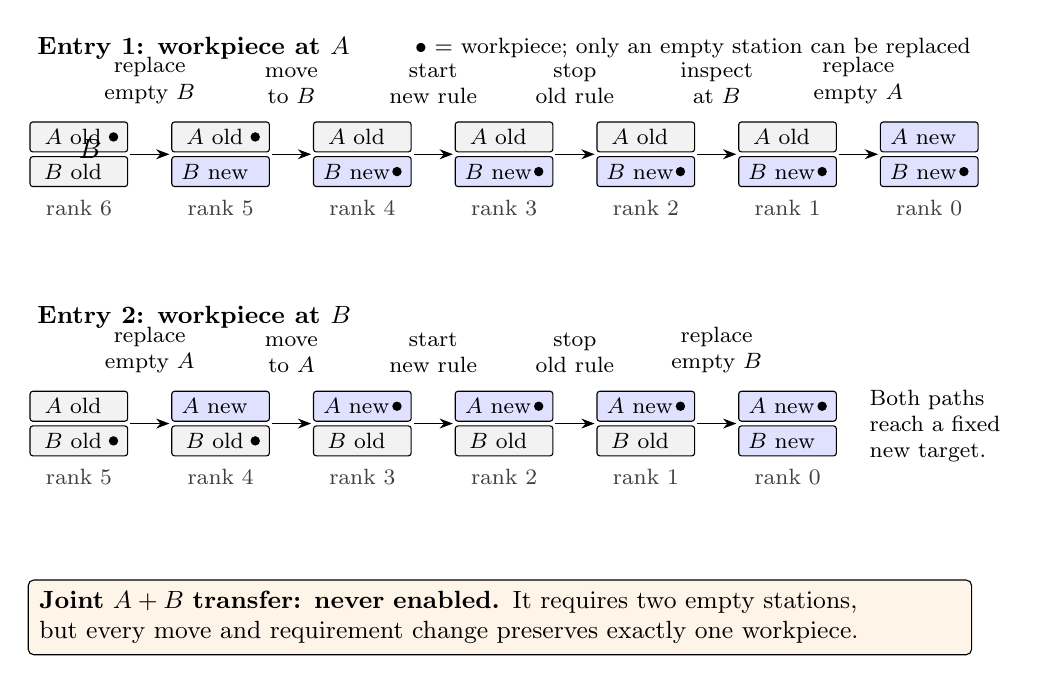
\begin{tikzpicture}[x=1cm,y=1cm,>=Stealth,
  station/.style={draw,rounded corners=1pt,minimum width=1.24cm,minimum height=.38cm,inner sep=1pt,font=\footnotesize,anchor=center},
  old/.style={station,fill=black!5},
  new/.style={station,fill=blue!12},
  action/.style={font=\footnotesize,align=center,anchor=south},
  ranklabel/.style={font=\footnotesize,text=black!75}]
\node[anchor=west,font=\small\bfseries] at (-.65,1.4) {Entry 1: workpiece at $A$};
\node[anchor=east,font=\footnotesize] at (11.45,1.4) {$\bullet$ = workpiece; only an empty station can be replaced};
\foreach \x/\av/\bv/\holder/\r in {0/old/old/A/6,1.8/old/new/A/5,3.6/old/new/B/4,5.4/old/new/B/3,7.2/old/new/B/2,9/old/new/B/1,10.8/new/new/B/0}{
  \node[\av] at (\x,.27) {$A$ \av\phantom{$\bullet$}};
  \node[\bv] at (\x,-.17) {$B$ \bv\phantom{$\bullet$}};
  \def\aholder{A}\ifx\holder\aholder
    \fill (\x+.44,.27) circle (1.7pt);
  \else
    \fill (\x+.44,-.17) circle (1.7pt);
  \fi
  \node[ranklabel] at (\x,-.63) {rank \r};
}
\foreach \left/\right/\word in {0/1.8/{replace\\empty $B$},1.8/3.6/{move\\to $B$},3.6/5.4/{start\\new rule},5.4/7.2/{stop\\old rule},7.2/9/{inspect\\at $B$},9/10.8/{replace\\empty $A$}}{
  \draw[->] (\left+.65,.05)--(\right-.65,.05);
  \node[action] at ({(\left+\right)/2},.57) {\word};
}
\CellRuleBand{-.62}{6.3}{-.91}{black!7}{Old rule: inspection forbidden}
\CellRuleBand{4.5}{8.1}{-1.32}{orange!13}{New: inspection pending}
\CellRuleBand{8.1}{11.42}{-1.32}{blue!10}{New: inspection clear}
\node[anchor=west,font=\small\bfseries] at (-.65,-2.02) {Entry 2: workpiece at $B$};
\begin{scope}[yshift=-3.42cm]
\foreach \x/\av/\bv/\holder/\r in {0/old/old/B/5,1.8/new/old/B/4,3.6/new/old/A/3,5.4/new/old/A/2,7.2/new/old/A/1,9/new/new/A/0}{
  \node[\av] at (\x,.27) {$A$ \av\phantom{$\bullet$}};
  \node[\bv] at (\x,-.17) {$B$ \bv\phantom{$\bullet$}};
  \def\aholder{A}\ifx\holder\aholder
    \fill (\x+.44,.27) circle (1.7pt);
  \else
    \fill (\x+.44,-.17) circle (1.7pt);
  \fi
  \node[ranklabel] at (\x,-.63) {rank \r};
}
\foreach \left/\right/\word in {0/1.8/{replace\\empty $A$},1.8/3.6/{move\\to $A$},3.6/5.4/{start\\new rule},5.4/7.2/{stop\\old rule},7.2/9/{replace\\empty $B$}}{
  \draw[->] (\left+.65,.05)--(\right-.65,.05);
  \node[action] at ({(\left+\right)/2},.57) {\word};
}
\node[align=left,anchor=west,font=\footnotesize] at (9.92,.02) {Both paths\\reach a fixed\\new target.};
\CellRuleBand{-.62}{6.3}{-.91}{black!7}{Old rule: inspection forbidden}
\CellRuleBand{4.5}{9.62}{-1.32}{blue!10}{New: clear ($B$ empty at new-start)}
\end{scope}
\node[draw,fill=orange!9,rounded corners=2pt,align=left,text width=11.7cm,inner sep=4pt,anchor=north west,font=\small] at (-.65,-5.35)
  {\textbf{Joint $A+B$ transfer: never enabled.} It requires two empty stations,\\but every move and requirement change preserves exactly one workpiece.};
\end{tikzpicture}
\caption{A complete local policy from both old entries. Bands mark active rules and new-rule inspection memory; new-start precedes old-stop. Each arrow has one action and one outcome, decreasing rank toward a fixed new target. Joint transfer merges these local commands with endpoints and requirements unchanged; this is not a DUCS encoding.}
\label{fig:cell-story}\label{tab:cell-story}
\Description{Two complete paths track the workpiece, station versions, active rules and inspection memory. From A holding: replace B, move to B, start the new rule with inspection pending, stop the old inspection ban, inspect at B to clear the new memory, replace A. From B holding: replace A, move to A, start the new rule already inspection-clear, stop the old rule, replace B. Both rules are active between new-start and old-stop. Ranks decrease from six and five to zero. A joint replacement is impossible because both stations can never be empty.}
\end{figure}


\paragraph{The generated policy.}
Figure~\ref{fig:cell-story} gives the whole policy. Starting with $A$ occupied, it replaces empty $B$, moves the workpiece to $B$, starts the new rule, stops the old rule, inspects, and replaces empty $A$. Starting with $B$ occupied, it first replaces $A$ and moves the workpiece there; the new rule then starts without an inspection debt. Every displayed event has one outcome and other controls are disabled.

The two paths contain 13 states and 11 edges. Their remaining lengths decrease from six or five to zero, proving completion as well as safety. A joint replacement cannot begin because it requires both stations empty. The example therefore shows why synthesis must coordinate local choices instead of merely check each endpoint. Technical Appendix~\ref{ta:cell} and S1 give the complete closure argument.

\Needspace{7\baselineskip}
\subsection{Audit and Role Lifetimes}
Policy(2) denotes this constructed example's two old/new requirement pairs: audit and access roles. Four bits record active rules $a_o,a_n,r_o,r_n$. The interval invariant $(a_o\lor a_n)\land\neg(r_o\land r_n)$ requires opposing boundary orders:
\[
\begin{array}{r@{\quad}c@{\;}c@{\;}c@{\;}c@{\;}c}
\text{Audit:}&\text{old only}&\xrightarrow{\text{new-start}}&\text{both active}&\xrightarrow{\text{old-stop}}&\text{new only}\\[2pt]
\text{Role:}&\text{old only}&\xrightarrow{\text{old-stop}}&\text{neither active}&\xrightarrow{\text{new-start}}&\text{new only}
\end{array}
\]
The role gap follows from the declared interval invariant; access monitors alone do not require it. The new audit monitor starts unlogged and requires a log before service. Each endpoint alternates its own log and service events and permits only its version's access role. With an identity component transfer, the saved policy first performs service if the old audit is logged, starts new audit, stops old audit and role, transfers, and starts the new role. Service is optional; this policy reaches a compatible new endpoint from both old states, with rank at most six.

If the starts are merged and the stops are merged, the first start overlaps roles and the first stop removes audit coverage. Ordinary events and transfer preserve the four activity bits, so neither old entry has a completing merged policy. Technical Appendix~\ref{ta:policy_interpretation} gives the complete finite input, policy and losing closure. This compares merged and separate FG-DUCS requirement boundaries.

\subsection{Existing Update Interfaces}
\label{sec:ducs-cell-construction}
\begin{table}[!htbp]
\centering\small
\caption{The formal workflow. Update control replaces old control; handover resumes the selected new controller.}
\label{tab:contract-workflow}
\begin{tabular}{@{}>{\raggedright\arraybackslash}p{.30\linewidth}@{\hspace{.05\linewidth}}>{\raggedright\arraybackslash}p{.30\linewidth}@{\hspace{.05\linewidth}}>{\raggedright\arraybackslash}p{.30\linewidth}@{}}\toprule
\textbf{Modeler supplies} & \textbf{Compiler generates} & \textbf{Synthesis returns}\\\midrule
Old/new components and fixed controllers; local transfer relations; requirement monitors, initializers and optional precedence; loadable endpoint states
& Mixed-version transitions, individual requirement boundaries, all old entries and compatible handover goals; no update sequence is supplied.
& Policy, decreasing rank and matched handover states covering every entry and outcome; otherwise a losing region excludes every policy.\\\bottomrule
\end{tabular}
\end{table}


\paragraph{Earlier endpoint reconnection.}
On-the-fly DUCS (O-DUCS) separates update and post-update analysis~\cite[Sec.~3]{HiranoEtAl2024ODUCS}. The archived fork in S4.8 synthesizes a new controller, matches component and new-safety states, and copies its transitions~\cite{FGDUCSAnonymousArtifact}. Identity with the 2024 release is unestablished.

\subsection{What the Local Interface Generates}
\label{sec:ducs-cell-construction}
Table~\ref{tab:main-generation} distinguishes the supplied structures from the generated result. DUCS already constructs an update environment and goal; GR(1) updating already constructs a bridge. From the supplied local contract, FG-DUCS constructs mixed-component transitions, implements individual monitor lifetimes, and derives handover target tests.

\begin{table}[!htbp]
\centering\small
\caption{Input and generation responsibilities. Existing guarantees are retained in the comparison; the rows do not claim a general translation or measured modeling-effort reduction.}
\label{tab:main-generation}
\begin{tabular}{@{}p{.16\linewidth}p{.36\linewidth}p{.43\linewidth}@{}}\toprule
Interface & Supplied structure & Generated result and guarantee\\\midrule
DUCS~\cite[Defs.~4.1--4.3, 5.1]{Nahabedian2020} & Environments/goals, old controller, global transfer, transition requirements and update fluents & Update environment/goal, update-and-subsequent controller and controller-transfer relation; legal, deadlock-free completion from every old-controller state\\
GR(1) update~\cite[Def.~3.1, Secs.~4--4.1]{Amram2022GR1DynamicUpdate} & Old/new specifications and switching condition & New controller, bridge and switching bookkeeping; bounded switching and new-specification satisfaction from winning states\\
FG-DUCS & Local components/transfers, requirement lifetimes/initializers and fixed endpoints & Mixed game and WIN/LOSS certificates; local-history correspondence and selected-endpoint continuation\\\bottomrule
\end{tabular}
\end{table}

\paragraph{Concrete Cell constructions.}
A native DUCS encoding supplies eight mixed version/holder stages and three endpoint states in $E'$, empty-station guards, history fluents for inspection/lifetimes, and a target gate. DUCS supplies its interrupt/protocol composition. Our explicit construction preserves both Cell paths and every endpoint continuation; its additional eventual-handover condition uses theoretical FLTL beyond native safety-$T$~\cite[Sec.~5.3]{Nahabedian2020}. The 11 states imply no lower bound (Technical Appendix~\ref{ta:ducs_cell_complete}).

For GR(1), supply version/lifetime predicates, $p'=[h=B]$ at start, inspection release at stop, and a target test. Unmodified old safety forbids inspection until global switching. Both paths are preserved; the algorithm adds \emph{switch}/\emph{allowed} bookkeeping and retains its chosen $C_2$ after the bridge. FG-DUCS takes endpoints as inputs and derives the local update structure. These analytical Cell witnesses are not solver runs or general translations (Technical Appendix~\ref{ta:gr1-cell}).


\section{Defining an Update Contract}
\label{sec:formalization}
\label{tab:contract-inputs}
\subsection{Supplied Choices}
The contract states what may change and what must be preserved. Its inputs are component models and transfers, requirements and their initializers, and fixed endpoint controllers. Synthesis supplies the coordination among them.

\paragraph{Finite transition systems and safety monitors.}
A labeled transition system (LTS) $\mathcal L=(S,\Sigma_{\mathcal L},\delta,s^0)$ has nondeterministic transitions $\delta:S\times\Sigma_{\mathcal L}\to2^S$. Partition events as $\Sigma=\Sigmauc\uplus\Sigmac$: controllers may disable controllables but cannot select outcomes or suppress uncontrollable (UC) events. A synchronous-product event requires a transition in every component whose alphabet contains it; other components retain their state~\cite{MageeKramer2006}.
A monitor is an automaton that checks a requirement as events occur. Requirement $r$ has a total deterministic monitor $t_r=(M_r,\Sigma,\eta_r,m_r^0,F_r)$ with absorbing errors for violating prefixes~\cite{AlpernSchneider1985,KupfermanVardi2001}. The empty monitor product has one non-error state. Monitors observe labels; policies also observe successor component states.

\label{def:fg-inputs}
\label{def:update_plan}
\paragraph{Components and transfers.}
For each $i\in I$, let $e_i^{\mathrm{old}},e_i^{\mathrm{new}}$ be the pre-update and post-update components and let $g_i\subseteq S_{e_i^{\mathrm{old}}}\times S_{e_i^{\mathrm{new}}}$ be their state-transfer relation.
  Define $g_i(s)=\{s'\mid(s,s')\in g_i\}$. The supplied $g_i$ includes every modeled transformation outcome. Let $E^v=\mathop{\parallel}_{i\in I}e_i^v$.

\paragraph{Requirements and activation.}
Let pairwise-disjoint $R^{\mathrm{old}},R^{\mathrm{new}},R^{\mathrm{upd}}$ contain the pre-update, post-update, and update-interval safety requirements, respectively.
For each $r\in R^{\mathrm{new}}\cup R^{\mathrm{upd}}$, the input supplies a partial \emph{monitor-initialization map} $\iota_r$ from version-tagged component tuples to $M_r\setminus F_r$. Its domain specifies where activation is allowed.
Section~\ref{sec:monitor-meaning} defines history-based and activation-scoped interpretations. For $r\in R^{\mathrm{upd}}$, $\operatorname{dom}\iota_r$ includes every reachable old component state.

\paragraph{Endpoints and handover targets.}
\label{def:endpoint_controllers}
For $v\in\{\mathrm{old},\mathrm{new}\}$, the supplied finite controller $C^v$ preserves uncontrollables and makes $E^v\parallel C^v$ deadlock-free and satisfy $R^v$. Hiding controller auxiliary events leaves observation alphabet $\bigcup_i\Sigma_{e_i^v}$; the union over both versions is the ordinary alphabet $\SigmaN$. Write $\Reach$ for initial-state reachability and
\[
\mathsf{CL}^v=E^v\parallel C^v\parallel\mathop{\parallel}_{r\in R^v}t_r.
\]
Monitors are passive: every endpoint transition originates in $E^v\parallel C^v$; a monitor only updates on that label and adds no enabled event.
The input supplies nonempty, checked targets $Z_{\mathrm{load}}\subseteq\Reach(\CLnew)$ with component, controller and new-monitor states.

\paragraph{Update commands and order.}
The set of update events, each executed exactly once, is
  \begin{equation}
  \SigmaU=
    \{\rho_i\mid i\in I\}
    \cup\{\ustop{r}\mid r\in R^{\mathrm{old}}\}
    \cup\{\ustart{r}\mid r\in R^{\mathrm{new}}\}.
  \end{equation}
These controllable events transfer components, stop old monitors or start new ones, respectively, and are disjoint from ordinary events $\SigmaN$:
$\Sigma=\SigmaN\uplus\SigmaU$ and $\SigmaU\subseteq\Sigmac$. Each transfer event $\rho_i$ is one atomic model transition: the controller chooses the update, but cannot choose its $g_i$ outcome.

An optional strict partial order $\prec\ \subseteq\SigmaU\times\SigmaU$ expresses precedence among update operations. For a pending-event set $P$, event $a$ is order-enabled exactly when $a\in P$ and every $a'\prec a$ has left $P$.
Monitors self-loop on update events that they do not specify.
\paragraph{Eligible contracts.}
An eligible contract satisfies the finiteness, typing, totality and non-error conditions above; dependencies form a strict partial order, and endpoint controller alphabets cover environment labels. Eligibility is structural; Section~\ref{sec:monitor-meaning} justifies initializer meanings.

\Needspace{4\baselineskip}
\subsection{States, Transitions, and Completion}
\label{sec:game-rules}

\label{def:configuration}
\label{def:init}
\emph{States and all entry states.}
An update state $q=(\xi,\mu,P)$ records each component's version/state $\xi(i)=(v,s)$ with $s\in S_{e_i^v}$, each monitor's state $\mu(t_r)\in M_r\cup\{\bot\}$ ($\bot$ means inactive), and pending commands $P\subseteq\SigmaU$.
Here $\rho_i\in P$ exactly when component $i$ is old. Old monitors remain active until their stop leaves $P$; new monitors become active when their start leaves $P$; update monitors are always active. 

Admission $\Init(z)$ copies $z$'s component and old-monitor states, installs interval initializers, leaves new monitors inactive and sets $P=\SigmaU$. The update policy replaces $C^{\mathrm{old}}$ and its scheduling restrictions. Declared old monitors remain until their stops; undeclared objectives, including old liveness, are not preserved. Duties needed throughout belong in interval monitors. The entry set is
\begin{equation}
 Q_0=\{\Init(z)\mid
 z\in\Reach(\mathsf{CL}^{\mathrm{old}})\}.
\label{eq:initial}
\end{equation}
All-entry coverage forbids waiting for a favorable old state.
\par\noindent\emph{Four kinds of induced transitions.}
\label{def:successor}
For $\xi(i)=(v,s)$, component $i$ uses $e_i^v$. The active-component product determines enabled ordinary uncontrollables $U(q)$, including those with unsafe outcomes, independently of updates and goals. For every $a\in\SigmaU$, impose
\begin{equation}
 U(q)\ne\emptyset\quad\Longrightarrow\quad\Post(q,a)=\emptyset.
 \label{eq:nonpreemption}
\end{equation}
Thus even a local command waits until the active-component product has no enabled uncontrollable event. A finite operation may drain to such a point; perpetual polling may prevent it. This global \emph{uncontrollable quiescence} differs from transaction quiescence~\cite{KramerMagee1990Quiescence} and tranquility~\cite{VandewoudeEtAl2007Tranquility}. Ordinary controls may coexist with UC. The following rules define $\Post$; unmentioned coordinates stay unchanged. ``Advance'' means $\mu'(t_r)=\eta_r(\mu(t_r),a)$ for the specified active monitors.

\begin{description}
  \item[Ordinary event $a\in\SigmaN$.]
  If $a$ belongs to the local event set of at least one active component and every active component having $a$ can transition, take every synchronous-product outcome and advance every active monitor.

  \item[Component update $\rho_i$.]
  If $U(q)=\emptyset$, order-enabled, and $\xi(i)=(\mathrm{old},s)$, set $\xi'(i)=(\mathrm{new},s')$ for each $s'\in g_i(s)$, delete $\rho_i$ from $P$, and advance every active monitor.

  \item[Requirement deactivation $\ustop{r}$.]
  If $U(q)=\emptyset$ and order-enabled, advance every active monitor except $t_r$, retain inactive monitors at $\bot$, set $\mu'(t_r)=\bot$, and delete $\ustop{r}$ from $P$; $t_r$ does not observe it.

  \item[Requirement activation $\ustart{r}$.]
  If $U(q)=\emptyset$, order-enabled, and $\xi\in\operatorname{dom}\iota_r$, advance every active monitor, retain other inactive monitors at $\bot$, install $\mu'(t_r)=\iota_r(\xi)$, and delete $\ustart{r}$ from $P$; $t_r$ begins online observation afterward.
\end{description}
If a precondition is false, the successor set is empty; every nondeterministic outcome is included and environment-chosen.
Let $\mathcal Q$ contain every state reachable from $Q_0$ through these transitions. 
\par\noindent\emph{Safety and handover-ready goals.}
\label{def:safe_goal}
An update state $q=(\xi,\mu,P)$ is safe, written $\Safe(q)$, exactly when every active monitor is outside its error states.
For $P=\emptyset$ and $z\in Z_{\mathrm{load}}$, write $q\sim z$ when component states (without version tags) and all new-monitor states agree. The handover map $\kappa$ selects such a full endpoint state $z$. Goals are
\begin{equation}
\Goal=\{q=(\xi,\mu,\emptyset)\in\mathcal Q\mid
\Safe(q)\land U(q)=\emptyset\land\exists z\in Z_{\mathrm{load}}:q\sim z\}.
\label{eq:goal}
\end{equation}
The goal is a quiescent handover boundary, not merely completion of the command list. At a goal, interval obligations end and matched new monitors continue. Handover disables ordinary controllables and installs $\kappa(q)$'s controller state, outside $\Sigma$ and the rank. UC cannot compete; compatible targets may have different continuations.
\par\noindent\emph{State-dependent policies and finite completion.}
\label{def:strategy}
A memoryless update policy is a function
$\sigma:\mathcal Q\setminus\Goal\to2^{\Sigmac}$ selecting only events with nonempty successor sets.

The possible next states under this policy are
\begin{equation}
 \SuccSet_\sigma(q)=
 \bigcup_{u\in U(q)}\Post(q,u)
 \ \cup\
 \bigcup_{a\in\sigma(q)}\Post(q,a).
\label{eq:strategy-successors}
\end{equation}
The environment chooses any uncontrollable and any permitted-event outcome. The returned policy retains one controllable at a quiescent state.

Let $\Reach_\sigma(Q_0)$ be the policy closure from $Q_0$, stopping at goals. 

\emph{Runs, winning, and witnesses.}
A run follows the policy successors and stops at a goal. It is \emph{maximal} if infinite or ending at a goal or a state without successors. A single policy $\sigma$ is winning for an FG-DUCS instance if, from every $q_0\in Q_0$,
(i) every reachable update state is safe, (ii) every reachable non-goal state has a successor, and
(iii) every maximal update run reaches $\Goal$ after finitely many events.
This \emph{finite completion} counts events and assumes no fairness. Winning policies exclude controllable self-loops during update; a reached UC self-loop makes a state losing. Ordinary actions can progress, as Cell's moves and inspection do. Handover restores the supplied controller's full matched behavior.

A \emph{progress-ranking function} for a winning policy is $\rank:\Reach_\sigma(Q_0)\to\mathbb N$, with value 0 at goal states and satisfying $\rank(q')<\rank(q)$ for every non-goal state $q$ and every
$q'\in \SuccSet_\sigma(q)$.

\paragraph{The FG-DUCS problem.}
Decide whether one policy safely completes the eligible game from every entry under every permitted event and outcome. Return $(\sigma,\rank,\kappa)$ covering all $Q_0$, or a losing-region certificate.

\subsection{Why the Generated State Represents the Contract}
\label{sec:contract-adequacy}
A \emph{local update history} $\ell=z(a_1,o_1)\cdots(a_n,o_n)$ begins at an old closed-loop tuple and records each event and its realized local successors. Components follow their active-version transitions and local transfers; boundaries preserve physical states. Monitor memories fold their active intervals: stop excludes its own boundary; start installs its initializer after the boundary. Initially inherit old memories, initialize interval monitors and release old control, leaving new monitors inactive.

Ordinary events retain all combinations of participating local outcomes. Commands require UC quiescence, unexecuted status, completed predecessors and a transfer/initializer value where applicable. Quiescence includes unsafe UC outcomes. A source policy selects controllable labels and must retain every UC and every permitted outcome. Every maximal history must safely reach a quiescent matching target after all commands. Technical Appendix~\ref{ta:source_synthesis} gives the full recurrences.

\begin{proposition}[Adequacy of the generated update game]
\label{prop:contract-adequacy}
For an eligible contract, map each local update history to its current component tuple, active monitor memories and unexecuted commands. Histories with the same image admit the same next events and all the same local outcomes, agree on safety, and have the same handover targets. This map gives a label- and outcome-preserving correspondence between local update histories and paths of the generated game. A history-dependent policy satisfying the source obligations exists exactly when a winning policy exists in that game.
\end{proposition}
\begin{proof}
Let $F(h)$ be the tuple obtained by folding the stated source operations over history $h$, with pending commands the complement of executed commands. At entry, $F(h)=\Init(z)$, giving exactly $Q_0$. Suppose a history ends at $(\xi,\mu,P)$. For an ordinary event, both descriptions require the same participating component edges, retain their full Cartesian product and advance every active monitor. For a transfer, both require quiescence, pending status, completed predecessors and an outcome of the same $g_i$; they change only component $i$, advance active monitors and consume that command. A stop removes its own monitor without consuming the boundary and advances the others. A start advances existing monitors and installs the same initializer, without a second observation. Thus each permitted label and each outcome has exactly the same successor image in both descriptions; no choice of outcome is introduced or removed. Quiescence counts unsafe UC outcomes in both. Safety and compatible targets depend on identical coordinates.

Induction gives a game path for every source history. Conversely choose an old tuple witnessing the first game state and lift each edge by the one-step property, retaining its outcome. The same recurrence lifts infinite paths. Histories with the same image admit identical future extensions because old control is released at entry. A game policy therefore lifts through $F$. Conversely, fix one old witness for each entry and consistently lift each game path from it; applying a source policy to that lifted history defines a game history-dependent policy. Both translations preserve every enabled UC event, every selected-label outcome, unsafe prefixes, deadlocks and infinite avoiding runs. Winning existence is therefore equivalent for history-dependent policies. Theorem~\ref{thm:correctness}'s losing-closure argument rules out every history-dependent winner on failure and returns a state-based winner on success, establishing the stated equivalence.
\end{proof}
This proves correspondence for the supplied contract; requirement meaning and Java frontend correctness remain separate obligations. Technical Appendix~\ref{ta:source_synthesis} gives the full source recurrences and expanded proof.

\begin{proposition}[Preservation of the selected endpoint]
\label{prop:endpoint-continuation}
For a returned winning-policy certificate and reached goal $q$, the new-phase submodel reachable after handover at $q$ is label-preserving isomorphic to $\CLnew$ rooted at $\kappa(q)$. Hence their finite and infinite ordinary-event traces coincide.
\end{proposition}
\begin{proof}
Handover retains matching components and monitors and installs the selected controller state. Each new-phase state copies an endpoint state with exactly its labeled transitions, without further policy restriction or return to updating. This bijection preserves and reflects edges, hence finite and infinite paths.
\end{proof}
Continuation properties established at the selected state are preserved; target selection can change which continuation applies.

\paragraph{Why matching and reconnection both matter.}
Cell's prefix $\rho_B,m_B,\mathsf{start},\mathsf{stop},\rho_A$ finishes every command with inspection pending. Physical matching alone admits clear target $z_B$, whose $m_A$ violates that duty; monitor matching excludes the reset. Conversely, disabling controllable loop $b$ in a one-state endpoint with loops $a,b$ and goal $\mathit{true}$ preserves legality, deadlock freedom and safety~\cite[Defs.~3.9--3.10, 4.3]{Nahabedian2020}, but loses $b$-continuations. FG's fixed-endpoint contract requires preserving those continuations.

Technical Appendix~\ref{ta:endpoint-interface} gives the endpoint interface and conditions for reusing a certificate when endpoints change.

\section{What a Winning Policy Guarantees}
\label{sec:interpretation-execution}
\label{sec:proof}
\label{sec:runtime-boundary}
The game proves safe completion for the supplied monitors. To understand what this means for a requirement, we must first identify the obligation installed when that monitor starts. We then state what is needed to carry the model guarantee into an execution. Table~\ref{tab:guarantee-evidence} provides this map.
\begin{table}[!htbp]
\caption{Guarantees and their evidence. Requirement interpretations are distinct; source checks alone do not establish actual activation conformance.}
\label{tab:guarantee-evidence}
\centering\small
\begin{tabular}{@{}p{.18\linewidth}p{.40\linewidth}p{.36\linewidth}@{}}\toprule
Scope & Established result & Remaining premise or boundary\\\midrule
Game & Safe finite completion from all entries; matching target & Supplied successor/endpoint predicates (Theorem~\ref{thm:correctness})\\
Invariant from start & Exact source language at 900 non-error cells in 138 lookup tables; direct PC2/GSM policy arguments & No benchmark-wide check of actual key/observation/fallback conformance\\
Safe prior histories & \RSNewOccurrences{} NEW residual inclusions & Nonempty scopes unverified except one PC2 tuple; empty scopes pass vacuously\\
From update entry & \VThreeRSUpdExact{} exact UPD initializations: 46 R1/89 R2 & Source guard/stage-fluent conditions; physical decoding remains unvalidated\\
Execution & Handover within the entry's event rank & A1--A4; platform conformance and elapsed-time bounds unvalidated\\\bottomrule
\end{tabular}
\par\smallskip{\footnotesize Cell's occupancy-based duty is proved in Section~\ref{sec:cell-activation-duty}. Whole-history obligations are not claimed: 39/126 PC2 entries admit a safe full prefix; 87 fail that check. Details: Technical Appendices~\ref{ta:history_checks} and~\ref{ta:lookup-act}.}
\end{table}


\subsection{Giving Requirements Their Intended Lifetimes}
\label{sec:monitor-meaning}
\paragraph{An exact activation obligation.}\label{sec:cell-activation-duty}
Cell's owed-inspection bit starts at 1 exactly when $B$ holds the workpiece. Event $m_B$ sets it, $j$ clears it, and $m_A$ is forbidden while it is 1; other labels preserve it. Encoding 0 by $c$ and 1 by $d$ makes every monitor transition identical to this rule, including rejection of forbidden departure. Initialization and suffix induction prove exact enforcement. Figure~\ref{fig:cell-story}'s first path starts with debt and clears it by ordinary inspection; the second starts clear.

\paragraph{When prior histories are part of the requirement.}
For prefix-closed requirement language $S_r$, declared activation histories $H_r(\xi)$ and monitor continuations $L_r(m)$, residual soundness (RS) means
$L_r(\iota_r(\xi))\subseteq\bigcap_{h\in H_r(\xi)}\{w:hw\in S_r\}$.
New histories include start once; monitors consume later events. Equality is exact; strict inclusion can reject feasible updates, and an empty history set makes inclusion vacuous. Scope completeness and intent are external obligations (Technical Appendix~\ref{ta:residual_formal}).

A \emph{fluent} records setting/resetting events. The saved checks use \textbf{A} for NEW (safe pre-activation histories consistent with the component observation) and \textbf{E} for UPD (reference beginning at entry). \textbf{H}, which counts prior violations too, is not claimed (S3).

Cell's pending initializer is exact for occupancy-based debt but conservative for a start-only reference that starts clear. Safe-history inclusion alone establishes neither the occupancy duty nor ACT.

\subsection{Execution and Handover}

The execution connection has four distinct premises (Technical Appendix~\ref{ta:execution_proof}):
\par\noindent\textbf{A1:} endpoint observations preserve component/monitor states and same-labeled endpoint edges.
\par\noindent\textbf{A2:} update control disables only unselected controllables, preserves every UC event/outcome, reports the successor and eventually observes a next event.
\par\noindent\textbf{A3:} commands start quiescently and finish atomically, finitely and failure-free with an observed modeled successor.
\par\noindent\textbf{A4:} entry observes/copies the actual old state; quiescent handover installs the selected compatible state, using finite failure-free linearizable boundaries~\cite{HerlihyWing1990}.

Under A1--A4, every execution maps to the linked model and reaches handover within the entry rank (Theorem~\ref{thm:realization}). History completeness places every actual activation history in its declared scope; the residual inclusion above then justifies that interpretation. A2 assumes eventual event progress, without fairness among enabled choices. Internal divergence and unobservable outcomes are excluded; rank bounds events, not time.

\section{How Granularity Changes Feasibility}
\label{sec:granularity-analysis}
Merging commands removes intermediate states. We show why this can either prevent or enable completion; Section~\ref{sec:rq2} evaluates the specified comparisons.

\paragraph{What is merged.}
Partition transfers, old stops and new starts separately into blocks. A transfer block $B\subseteq I$ simultaneously permits all targets in $\prod_{i\in B}g_i(s_i)$; a boundary block removes or initializes its monitors at the same component tuple. Other active monitors compose member-label effects, checked to commute pairwise on every monitor/residual state. Mapped precedence must remain irreflexive and acyclic. Ordinary behavior, entries, endpoints, relations, initializers and targets stay fixed; quiescence and all member guards apply. These are comparison contracts, not DUCS encodings.

\begin{lemma}[Mandatory-command obstruction]
\label{lem:mandatory-obstruction}
Let $q_0$ be an entry and $B$ a nonempty set of commands pending there. Suppose a safe region $R$ contains $q_0$, retains all commands in $B$, and is closed under every safe successor whose label is outside $B$. If each command in $B$ is disabled or has an unsafe outcome at every state in $R$, no winning policy covers $q_0$.
\end{lemma}
\begin{proof}
Every goal exhausts pending commands, so a winner must execute a first command in $B$. Safety and closure keep its prefix in $R$, where that step is disabled or has an environment-chosen unsafe outcome. Avoiding it yields a non-goal deadlock or infinite run, also losing.
\end{proof}
In Cell's one-workpiece region, joint transfer is disabled; Policy retains its initial active bits until either grouped boundary violates the interval; PC2-Rolling's enabled joint transfer violates availability (Section~\ref{sec:pc2-case}). These results concern specified merges, not native DUCS expressiveness.


\paragraph{A capacity boundary.}
Readiness gates motivate the constructed Rolling contract~\cite{e6_kubernetes_deployments,e6_mongodb_enterprise_replica_set}. It starts with $n$ ready replicas, no spares, and an interval floor of $m$ ready replicas. A transfer boots its replicas; each becomes ready after one UC event, with no waiting loop. Service self-loops are controllable. The all-new, ready target restores capacity; service may pause during the update.

\begin{proposition}[Rolling threshold]\label{prop:rolling-threshold}
For $n\ge2$, $1\le m<n$ and $1\le k\le n$, fixed consecutive batches of size $k$ (with a smaller final remainder) admit safe finite completion iff $k\le n-m$.
\end{proposition}
\begin{proof}
Some mandatory batch has size $k$. Its transfer leaves at most $n-k$ ready replicas, so $k>n-m$ violates the interval. Otherwise, transfer one batch only when all replicas are ready, disable service, and retain every UC readiness outcome before the next transfer. Readiness never falls below $n-k\ge m$. With $u$ old and $b$ booting replicas, $2u+b$ strictly decreases on every selected transfer and every UC event, reaching zero exactly at the target. Thus all maximal runs finish without fairness.
\end{proof}

\paragraph{Why finer is not always better.}
Two components with one state per version share alphabet $\{x,y,tick\}$, with $x,y$ UC and $tick$ controllable. The only UC loops are $y$ in old~1, $x$ in new~1, $x$ in old~2 and $y$ in new~2; shared labels synchronize. Thus all-old and all-new are quiescent, but either mixed product has a UC loop. With identity transfers and no requirements, either first local transfer prevents quiescence forever, so fine loses. A joint transfer skips the mixed state and wins at rank one. Every version has a $tick$ loop, making both endpoints deadlock-free. Atomicity can therefore remove either a necessary or a harmful intermediate state; there is no general refinement order (Technical Appendix~\ref{ta:granularity-reverse}).
\section{Synthesizing and Checking an Update Policy}
The procedure specializes strong-planning and on-the-fly reachability principles~\cite{Cimatti1998StrongPlanning,TripakisAltisen1999,CiolekDCS}, retaining every queried event outcome and producing evidence for every old entry.
\label{sec:algorithm}

A \emph{bucket} is $\Post(q,a)$; empty means disabled. Disabling controls at a UC-enabled state removes runs without creating deadlock, preserving winning (\emph{UC priority}, Lemma~\ref{lem:uc-priority}). With quiescent goals and no fairness or controller priority, permitting commands while UC is enabled therefore adds no winning entries. Changing fairness or priority changes the game. The proof establishes memoryless sufficiency.

\subsection{Lazy Successor Generation}
Algorithm~\ref{alg:otf} constructs a reachability attractor~\cite{CassezEtAl2005TimedGames}. $V$ contains discovered states, $X$ those with all UC candidates queried, and $W$ proved winners. A UC state needs all successors to win; a quiescent state needs one complete control bucket. Lazy queries controls incrementally, keeping unfinished cursors in $\mathsf{Retry}$. Each promotion records a complete nonempty proving set and a rank above its members. Reverse incidences propagate promotions. Failure requires exhausted candidates and a promotion fixed point. Extraction chooses lower-rank controls and compatible targets; it need not minimize path length.

\SetAlgoNlRelativeSize{-1}
\SetAlgoRefRelativeSize{-1}
\begin{algorithm}[!htbp]
\caption{Lazy}
\label{alg:otf}
\footnotesize
\KwIn{Typed update contract (Section~\ref{sec:formalization})}
\KwOut{$(\sigma,\rank,\kappa)$ or $(\textnormal{no solution},L)$}
$V\leftarrow Q_0$; $X,\mathsf{Retry}\leftarrow\emptyset$; $W\leftarrow V\cap\Goal$\;
$\mathsf{Open}\leftarrow\{q\in Q_0\mid\Safe(q)\land q\notin\Goal\}$; set $\rank(q)\leftarrow0$ for $q\in W$\;
\While{true}{
  Add queued goals to $W$ once with rank zero; exhaust \emph{Promote}, retaining witnesses/ranks, removing winners from Retry and propagating predecessors\;
  \lIf{$Q_0\subseteq W$}{\Return $(\sigma,\rank|_{\Reach_\sigma(Q_0)},\kappa)$ constructed from the goal witnesses and retained lower-rank choices}
  \eIf{$\mathsf{Open}\neq\emptyset$}{
    Remove $q$ from $\mathsf{Open}$, add it to $X$, and query all uncontrollable candidates\;
    Close the control cursor if UC-enabled; otherwise initialize it and query to the next nonempty bucket or exhaustion\;
    Insert $q$ into $\mathsf{Retry}$ iff $q\notin W$ and its cursor has remaining candidates\;
  }{
    \lIf{$\mathsf{Retry}=\emptyset$}{\Return $(\textnormal{no solution},L\leftarrow V\setminus W)$}
    Remove $q$ from $\mathsf{Retry}$; query to the next nonempty bucket or exhaustion; reinsert iff $q\notin W$ and its cursor has remaining candidates\;
  }
  Add every queried successor to $V$; queue newly discovered goals for rank zero and safe non-goals for $\mathsf{Open}$ (unsafe states stay outside $W$ and $\mathsf{Open}$)\;
}
\end{algorithm}
\SetAlgoNlRelativeSize{-2}
\SetAlgoRefRelativeSize{-2}



\Needspace{9\baselineskip}
\subsection{Correctness and Certificates}




\begin{theorem}[Termination, soundness, and completeness]
\label{thm:correctness}
\label{thm:termination}
\label{thm:soundness}
\label{thm:completeness}
For every eligible finite FG-DUCS instance with Equation~\eqref{eq:nonpreemption} and quiescent goals in Equation~\eqref{eq:goal}, Algorithm~\ref{alg:otf} terminates. A returned $(\sigma,\rank,\kappa)$ keeps every active monitor non-error, preserves every uncontrollable event and every outcome of each policy event, reaches $\Goal$ finitely without deadlock, and gives each reached goal a compatible target in $Z_{\mathrm{load}}$ for the supplied game. It returns no solution iff no winning policy covers $Q_0$ in that supplied game.
\end{theorem}



\begin{proof}
\emph{Coverage and termination.} Every discovered safe non-goal enters $\mathsf{Open}$ until expansion queries all UC candidates. At quiescence, unfinished nonwinners retain their control cursors in $\mathsf{Retry}$; promotion removes only winners. Each state is expanded and promoted at most once, each candidate queried once, and reverse incidences processed on promotion. Finiteness therefore ensures termination and complete candidate coverage at failure.

\emph{Soundness.} Goals receive rank zero and compatible handover states. Each promotion adds a safe state above a complete nonempty set of ranked winners: all UC successors, or every outcome of one control event at quiescence. Buckets are immutable. Extraction retains those outcomes and disables other controls. Thus every reached non-goal is safe, has a successor, and strictly decreases a natural-number rank on every outcome. All maximal runs reach a matching quiescent goal. The monitor rules advance exactly the active memories, so induction from entry establishes every declared safety interval and preserves matching new memories at handover.

\emph{Completeness.} At failure both queues are empty and promotion has reached a fixed point. Some entry lies in goal-free $L=V\setminus W$. Coverage ensures that each safe state in $L$ was expanded. If UC-enabled, it has an outcome in $L$; otherwise it would have been promoted. At quiescence every control candidate is exhausted, and each enabled bucket likewise has an outcome in $L$. Against any history-dependent policy, the environment can keep selecting such outcomes. Disabling all events deadlocks; otherwise execution becomes unsafe or avoids goals forever. No winner covers that entry. A winning policy therefore excludes failure and forces success. The UC-priority lemma preserves winning when optional controls at UC-enabled states are removed.
\end{proof}


\paragraph{Checking the returned evidence.}
For WIN, let $D_\sigma=\Reach_\sigma(Q_0)$. The checker requires exactly $D_\sigma$ as the rank domain, safety throughout it and, at every non-goal, enabled selected controls, nonempty successor sets inside it, and strict rank decrease for every outcome. At goals it checks rank zero, UC quiescence and compatible $\kappa(q)\in Z_{\rm load}$, with $\operatorname{dom}\kappa=D_\sigma\cap\Goal$; omitted policy entries are empty.

For LOSS, $L\subseteq\mathcal Q$ must include an entry state and exclude all goals. Every safe $q\in L$ must have some UC outcome in $L$ when UC is enabled; otherwise every enabled controllable must have an outcome in $L$. Unsafe states and non-goal deadlocks lose. These conditions certify search relative to shared $\Post$ and endpoint predicates~\cite{HofmannEtAl2016MuCertificates}; the implementation and independent checks in the main paper state the trust boundary (Section~\ref{sec:evaluation}).




\subsection{Exploring the Compiled Contract on Demand}
\label{sec:exploration-unit}
\label{thm:lazy-separation}
With indexed predicates and constant-time bookkeeping, search is linear in discovered states, queried candidates and returned outcomes. This excludes preprocessing and Java sorting/scans; the reachable graph may be explored completely. Technical Appendix~\ref{ta:exploration_order} gives the accounting.

\section{Implementation and Evaluation}
\label{sec:evaluation}
\subsection{Design and Implementation}

RQ1 tests granularity mechanisms; RQ2 checks games, certificates and source monitors; RQ3 compares exploration and cost on \ApplicationContracts{} adapted contracts. Auxiliary trials remain outside fixed-budget medians.

Each of the \ApplicationModels{} inherited inputs has Base (no interval requirement) and alternative R1/R2 contracts. R1 blocks designated operational actions while flags set by any old-stop and cleared by their designated new-start are true. R2 requires selected old-stop/new-start events before their associated transfers. Actions and event pairs vary by model (S4). The separate PC2-Rolling case adds rolling calibration to a two-arm production cell. Legacy also synthesizes subsequent control and therefore solves a different objective.

\paragraph{Implementation.}
Our Modal Transition System Analyser (MTSA) extension~\cite{paper:MTSA2008} checks certificates~\cite{McConnellEtAl2011Certifying}; its composition checker, Link, checks the connected old, update and new controllers, including entries and targets. An independent oracle parses restricted Finite State Processes (FSP). Finite-JSON runs save losing membership; FSP benchmarks report only its statistics.

\paragraph{Use of generative AI}
Generative AI assisted the research design and proof drafting, the Java solver and frontend, and the Python checkers and experiment drivers. It also assisted experiment execution, analysis and manuscript editing. We validated the results through certificate and exhaustive checks, source/automaton comparisons, saved-output checks for tables, and primary-source checks for citations. Authors retain responsibility; correlated faults from shared AI and code remain a threat. Technical Appendix~\ref{ta:implementation_details} gives the tool roles.

\paragraph{Constructing the benchmark inputs.}
Nine inputs adapt eight DUCS sources; the one-arm and two-arm production-cell variants (PC1 and PC2) share a parent. PC1/PC2 preserve its repeatable, state-gated arrivals while making tool results UC. With work/output withheld, pending tool results and reset/arrival chains finish in quiescent arm states. Other adaptations shorten Railcab transfers while preserving both outcomes, omit a duplicate initial-environment transfer declaration in PowerPlant, and change safety or ordering. Technical Appendix~\ref{ta:additional_populations} details these changes; equivalence is unestablished.

MTSA compiles the FSP declarations into fixed endpoints, monitors and initializer tables before exploration. Every reachable new-endpoint state is admitted. The tables combine physical states with observer values; Cell instead supplies its initializer maps directly. S3 gives the construction, and S4 retains preparation times and tuple counts for all 27 contracts.

% FGDUCS_RELOCATED: benchmark_inputs

Only Railcab transfers branch; none of the inherited inputs declares precedence. R2 instead encodes order in monitors (Technical Appendix~\ref{ta:benchmark_inputs}).

\paragraph{Exploration variants.}
All methods share entries, successors, goals, checks and terminals. On-the-fly (OTF) variants omit controls at UC-enabled states and stop when all entries win. Direct-Full constructs all reachable buckets, including those controls, then applies UC priority; auxiliary Full+UC omits them during construction. At quiescence, Lazy queries individual buckets, Eager all controls; Update-first tests O-DUCS's update priority~\cite{HiranoEtAl2024ODUCS} within our solver. The query order gives priority to pending stops and transfers, and to starts after endpoint alignment. It guides exploration rather than requiring that execution order. Technical Appendix~\ref{ta:exploration_order} gives the conditional priorities, queues and tie rules.

\paragraph{Design and measures.}
RQ3 uses one Windows/Xeon host, a 64~GiB heap and a 1,200~s Java Virtual Machine (JVM) cap. Each timing median requires five completions; incomplete cells retain their capped trial. Solver time includes checking, while total JVM time also includes preparation, startup and output. Exploration, policy size and peak working set provide complementary measures. Full settings, Legacy's distinct timer, excluded Mac pilots and interruptions are retained in Technical Appendices~\ref{ta:implementation_details} and~\ref{ta:memory_policies} and S4.

\subsection{RQ1: Can Local Choices Change Feasibility?}
\label{sec:claim-granularity}
\label{sec:rq2}
We compare inherited inputs, constructed families and a source-derived case under Section~\ref{sec:granularity-analysis}'s merging rules. These comparisons do not estimate deployed prevalence.

\paragraph{Inherited inputs: no observed change.}
On nine inherited inputs, merging transfers, boundaries or both changes \VThreeEOneChanged{}/\VThreeEOneTrials{} Base/R1 decisions. Their total raw transfers omit Rolling's startup phase; totality alone does not ensure safe merging. States decrease in \VThreeEOneStatesReduced{} comparisons and stay equal in \VThreeEOneStatesEqual{}. R2 names individual events and is excluded. This null result limits observed granularity benefits.

\paragraph{Constructed mechanisms.}
The families isolate local choices, retaining both-WIN and both-LOSS controls.

Table~\ref{tab:rq2-family-counts} records \VThreeESixWitness{}/\VThreeESixMainPairs{} fine-WIN/merged-LOSS comparisons across five constructed families. Of the 33 separations, 30 are Rolling/Canary parameter points, not independent mechanisms. Rolling compares $k=1$ with $k=n$; its \VThreeESixRollingThresholdCells{} threshold cells are separate. Threads tests both-WIN/both-LOSS quiescence controls. Technical Appendix~\ref{ta:constructed_contracts} gives all definitions and assumption controls.

\textbf{Answer.} Separate commands can preserve capacity, necessary intermediate stages and compatible requirement lifetimes. Merging can instead bypass a harmful mixed state (Section~\ref{sec:granularity-analysis}); finer is not uniformly better. Inherited decisions do not change. PC2's source proof establishes merged impossibility, but its merged timeout leaves the solver comparison incomplete.

% Generated by scripts/generate_rq2_family_table.py; do not edit numeric cells.
\begin{table}[!htbp]
\caption{Constructed granularity comparisons: each pair fixes one model and compares its fine and merged contracts. Policy merges boundaries; other rows merge transfers. $n$ counts replicas/workers/stations. Canary bounds reported failures by $n-m$; otherwise $m$ is an availability floor. The main total excludes Cell.}
\label{tab:rq2-family-counts}
\centering\small
\begin{tabular}{@{}lp{.30\linewidth}rrrrr@{}}\toprule
Family / control & Parameter domain & Pairs & \shortstack{WIN /\\LOSS} & \shortstack{LOSS /\\LOSS} & \shortstack{WIN /\\WIN} & Inc.\\\midrule
Rolling & $n=2\ldots6,\ 1\le m<n$ & 15 & 15 & 0 & 0 & 0\\
Canary & $n=2\ldots6,\ 1\le m<n$ & 15 & 15 & 0 & 0 & 0\\
Policy & 2 rule pairs & 1 & 1 & 0 & 0 & 0\\
DB-Rolling & $n=3,\ m=2,3$ & 2 & 1 & 1 & 0 & 0\\
Rolling+Audit & $n=2,\ m=1$; 1 audit pair & 1 & 1 & 0 & 0 & 0\\
Threads (control) & $n=2\ldots6$; queue 1,2 & 20 & 0 & 10 & 10 & 0\\
PC2-Rolling & 2 arms; floor 1 & 1 & 0 & 0 & 0 & 1\\
\midrule
Main total &  & \VThreeESixMainPairs{} & \VThreeESixWitness{} & \VThreeESixBothLoss{} & \VThreeESixBothWin{} & \VThreeESixIncomplete{}\\
\midrule
Cell$_n$ (reference) & $n=2\ldots10$ & 9 & 9 & 0 & 0 & 0\\\bottomrule
\end{tabular}
\par\smallskip\raggedright\small Completed columns read fine / merged; Inc. denotes unresolved. PC2's merged solver remains TO, not LOSS. Threads is a negative control; its queue capacities are 1 and 2, with both backpressure and saturated-offer regimes.
Rolling+Audit counts transfer merging; boundary merging remains WIN and adds no pair here.
\end{table}


\Needspace{4\baselineskip}
\subsubsection{A Source-Derived Calibration Case}\label{sec:pc2-case}
PC2-Rolling adds calibration while requiring another arm operational. Requests are controllable, completions UC, and transfers enter calibration while preserving initializer observers. Erasing calibration recovers the original operational process, without whole-problem equivalence. Endpoints retain baseline requirements plus availability; the interval additionally treats transfers as calibration entry. The 25 boundaries and two transfers have no supplied order (Technical Appendix~\ref{ta:pc2-generation}).

The saved policy calibrates the arms in sequence, waiting for each completion. Technical Appendix~\ref{ta:pc2_history_boundary} shows one representative path; it does not prescribe a unique order for all policy branches. All \PCTwoCaseEntries{} entries are covered, every outcome decreases rank from at most \PCTwoCaseMaxRank{}, and at least \PCTwoCaseMinOperationalArms{} arm stays outside calibration. Link checks the full composition. Each of the thirteen source invariants holds at its start and through the remaining start-only suffix until handover, proving ACT on reached tuples. This covers neither all initializer tuples nor all 138 occurrences; GSM below exercises ordinary actions under an active new requirement.

Whole-history obligations give a different result: only 39/126 entries admit a safe full prefix; 87 fail. Every entry also admits an earlier violating cycle that restores zero observers. Technical Appendix~\ref{ta:pc2_history_boundary} preserves the complete failure partition and 38,288 initializer tuples whose safe-history nonemptiness remains unchecked.

\paragraph{Why the fixed merge loses.}
Every old entry admits both raw transfers. Before joint transfer, old plants lack calibration actions and all other steps preserve readiness. The joint transfer therefore puts both arms in calibration, clearing both interval readiness bits and reaching error. This proves impossibility, while the merged solver and fine Direct-Full both time out at \VThreeESixPCTwoCap{}~s/\VThreeESixPCTwoHeap{}~GiB. Those timeouts remain unresolved solver results.

Restricted-transfer comparisons also retain both-LOSS and incomplete cases (Technical Appendix~\ref{ta:additional_populations}; S1--S4).

\Needspace{7\baselineskip}
\subsection{RQ2: What Do the Checks Establish?}
\label{sec:claim-checks}
\label{sec:rq1}


\textbf{Answer.} Table~\ref{tab:validation-populations} maps the checks and their populations to the guarantee layers in Table~\ref{tab:guarantee-evidence}.
\begin{table}[!htbp]
\caption{RQ2 validation populations, keyed to the scopes in main-paper Table~\ref{tab:guarantee-routes}.}
\label{tab:validation-populations}
\centering\small
\begin{tabular}{@{}>{\raggedright\arraybackslash}p{.21\linewidth}>{\raggedright\arraybackslash}p{.30\linewidth}>{\raggedright\arraybackslash}p{.43\linewidth}@{}}\toprule
Scope and check & Population & Established result and boundary\\\midrule
Game:\newline independent games & \FixedRQOneFixtures{} fixtures, two solvers: \FixedRQOneJobs{} jobs & \FixedRQOneWin{} WIN, \FixedRQOneLoss{} LOSS, \FixedRQOneInvalid{} invalid; all \FixedRQOneEligible{} eligible jobs pass certificate/exhaustive checks.\\\addlinespace
Invariant from start:\newline New-requirement lookup tables & 46 source positions, 138 occurrences; 900 non-error cells & Exact start-scoped languages under reference observations (Proposition~\ref{prop:lookup-act}); general activation conformance remains a premise.\\\addlinespace
Invariant from start:\newline Saved Railcab policies & Base/R1: 22 entries each, 21 start edges; shared post graph & Source-observer replay and truth checks on all saved continuations; accepts exported entry vectors, excludes runtime/fallback (Appendix~\ref{ta:railcab-activation}).\\\addlinespace
From update entry:\newline Interval initialization & \VThreeRSUpdExact{} occurrences: 46 R1, 89 R2 & Exact entry-scoped initialization under reference observations; adapter conformance unchecked.\\\addlinespace
Game:\newline application policies & \FixedPolicies{} Lazy WIN contracts; 125 runs & Certificates check the shared Java game. Runs save summaries; complete PC2-Rolling/Railcab exports are separate.\\\bottomrule
\end{tabular}
\end{table}


\paragraph{What is checked independently.}\label{tab:validation-scope}
The \FixedRQOneJobs{}-job suite reconstructs explicit successors in Python and compares the resulting games with the solver. Every winning job passes the composition check; deliberately invalid cases omit events, deadlock or suppress uncontrollable behavior. \FixedTargetQuiescenceFixturesWord{} separate monitor-free fixtures reconstructs the FSP endpoints, games and goals (S4.2). The larger suite shares frontend and endpoint/goal code, so its independence covers successor construction rather than the entire translation.

\paragraph{What the requirement checks establish.}
For source invariants, initial truth and transition checks establish that the monitor follows the reference observation rules. Safe lookup reachability then supplies Proposition~\ref{prop:lookup-act}'s premise. Table~\ref{tab:validation-populations} gives the distinct populations: source positions, requirement occurrences, lookup cells and saved runs.

These checks leave one connection open: whether actual activation decodes the state correctly, chooses the post-start key, follows the same observation rules and avoids fallback initialization. In particular, the adapter retains physical observers across commands while reference action predicates can reset. Conservativeness of that difference is unproved. The checks therefore establish the recorded reference semantics, rather than source semantics for every winning application policy.

For the \RSNewOccurrences{} new-requirement occurrences, a separate inclusion check preserves obligations from admitted safe prior histories. Nonemptiness of the actual history scope remains unchecked except for one PC2 tuple. Update-interval requirements begin their reference at update entry. Technical Appendices~\ref{ta:lookup-act} and~\ref{ta:history_checks} give the full checks and interpretation conditions.

\paragraph{Source obligation over ordinary actions.}
\label{sec:gsm-entry-derivation}
GSM changes $\Box\neg decode.3$ to $\Box\neg decode.2$. From every old entry, reach the first $\mathsf{RECEIVED}$ state; then
\[
\mathsf{RECEIVED}\xrightarrow{stop,start}\mathsf{RECEIVED}
\xrightarrow{decode.3}\mathsf{DECODED}\xrightarrow{output}
\mathsf{SENDER}\xrightarrow{\rho}\mathsf{SENDER}_{new}.
\]
The preceding $receive$ sets the $decode.2$ observer to zero; boundaries preserve it. The saved initializer maps zero to monitor state zero: $decode.2$ enters error, all other labels preserve zero. Thus the new obligation constrains an actual ordinary choice. Transfer matches sender, observer and new-monitor zero to the endpoint. The pre-stop distance is at most seven; adding the five displayed events gives rank at most twelve. Consecutive stop/start satisfies R1's gap ban. This source-derived analytical policy proves ACT, not a new solver result; a separate 45-pair source check establishes E initialization (Technical Appendix~\ref{ta:activation_scope}).


% FGDUCS_RELOCATED: history_checks

\paragraph{What application WIN and LOSS mean.}\label{sec:railcab-policy}\label{sec:contract-case}
Railcab's Base policy covers 22 entries with 1--4 ordinary gap events; R1's has none and retains seven interval guards. Both pass certificate/Link. Gap duties require interval requirements; WIN alone supplies none (Technical Appendix~\ref{ta:saved-gaps}).

Railcab also illustrates branching: one milestone transfer has two possible results, requiring eleven or twelve further events to reach different new-controller states. The policy completes from both, rather than selecting a favorable outcome (S4.4.3).

Exhaustive closure shows Industry/R1 loses at \FixedIndustryLosingEntries{}/\FixedIndustryEntries{} entries under every order. Some workflow-validation actions violate the new monitors. The remaining document-review process permits endless rejection, or reaches a quiescent deadlock if safe validation is withheld. Native DUCS wins its different subsequent-control problem (Technical Appendix~\ref{ta:additional_populations}; S4).

% The complete trap figure remains in the candidate source; the main text states its obstruction.

\subsection{RQ3: Does Lazy Reduce Exploration?}
\label{sec:granularity-unit}
\label{sec:rq3}


\textbf{Answer.} With the same UC pruning, Lazy decides \FixedLazyDecisions{} contracts to Eager's \FixedEagerDecisions{}. Direct-Full additionally changes pruning and decides \FixedDirectFullDecisions{}; Lazy reduces states and queries in all \FixedDirectFullPairs{} completed pairs. All paired decisions agree (Table~\ref{tab:xeon-rq3}). Update-first is faster on \FixedUpdateFirstFaster{}/\FixedUpdateFirstPairs{} paired solver medians but adds \FixedUpdateFirstAdditionalTOWord{} timeouts. Lazy returns LOSS for Industry/R1 and times out on PC2/R2 at 1,200~s/64~GiB (fixed), 3,600~s/64~GiB (sensitivity) and 7,200~s/200~GiB (S4, earlier series); the limiting resource is unknown.

Legacy yields \LegacyNativeWins{} WIN, \LegacyNativeOOM{} OOM and \LegacyCaptureNM{} unmeasured snapshot-cap cases. Its differing subsequent-control objective precludes same-game ratios or impossibility inferences; endpoint preservation was not compared (Technical Appendix~\ref{ta:additional_populations}).



\begin{table}[!htbp]
\caption{All \ApplicationContracts{} contracts per method. TO denotes one capped trial, not a timing median. Ratios summarize heterogeneous completed pairs; values above one favor Lazy.}
\label{tab:xeon-rq3}\label{tab:paired-costs}
\centering\small
\begin{tabular}{@{}lrrrr@{}}\toprule
Method & WIN/LOSS/TO & Faster / pairs & Solver ratio & Total JVM ratio\\\midrule
Lazy & \FixedLazyOutcomes{} & --- & --- & ---\\
Eager & \FixedEagerOutcomes{} & \FixedEagerFaster{} / \FixedEagerPairs{} & \FixedEagerSolverRatio{} & \FixedEagerJVMRatio{}\\
Update-first & \FixedUpdateFirstOutcomes{} & \FixedUpdateFirstFaster{} / \FixedUpdateFirstPairs{} & \FixedUpdateFirstSolverRatio{} & \FixedUpdateFirstJVMRatio{}\\
Direct-Full & \FixedDirectFullOutcomes{}$^{\dagger}$ & \FixedDirectFullFaster{} / \FixedDirectFullPairs{} & \FixedDirectFullSolverRatio{} & \FixedDirectFullJVMRatio{}\\\bottomrule
\end{tabular}
\par\smallskip{\footnotesize TO: timeout; no OOM/unmeasured cases. $\dagger$ Workflow/R2 retains its interruption and later same-setting timeout (S4). Comparator/Lazy ratios are median [min--max] across completed pairs of five-run medians. Faster / pairs counts lower comparator solver medians among all completed pairs. JVM includes frontend, startup, endpoints and output; solver includes checking. Unresolved costs have no ratio.}
\end{table}

Figure~\ref{fig:rq3-paired-absolute} shows all 14 completed pairs (Technical Appendix~\ref{ta:workload_rows}). Base/R1/R2 contribute 5/3/6 pairs with median Direct-Full/Lazy state ratios 111.89/11.88/2.75. These different populations neither isolate interval effects nor attribute savings to old-stop/new-start gaps. In R2, Update-first has fewer states and lower solver medians in six of eight pairs (Technical Appendix~\ref{ta:additional_populations}).

% Generated from the unchanged rq3-cells.csv. All 27 contracts appear.
\begin{figure}[!htbp]
\centering
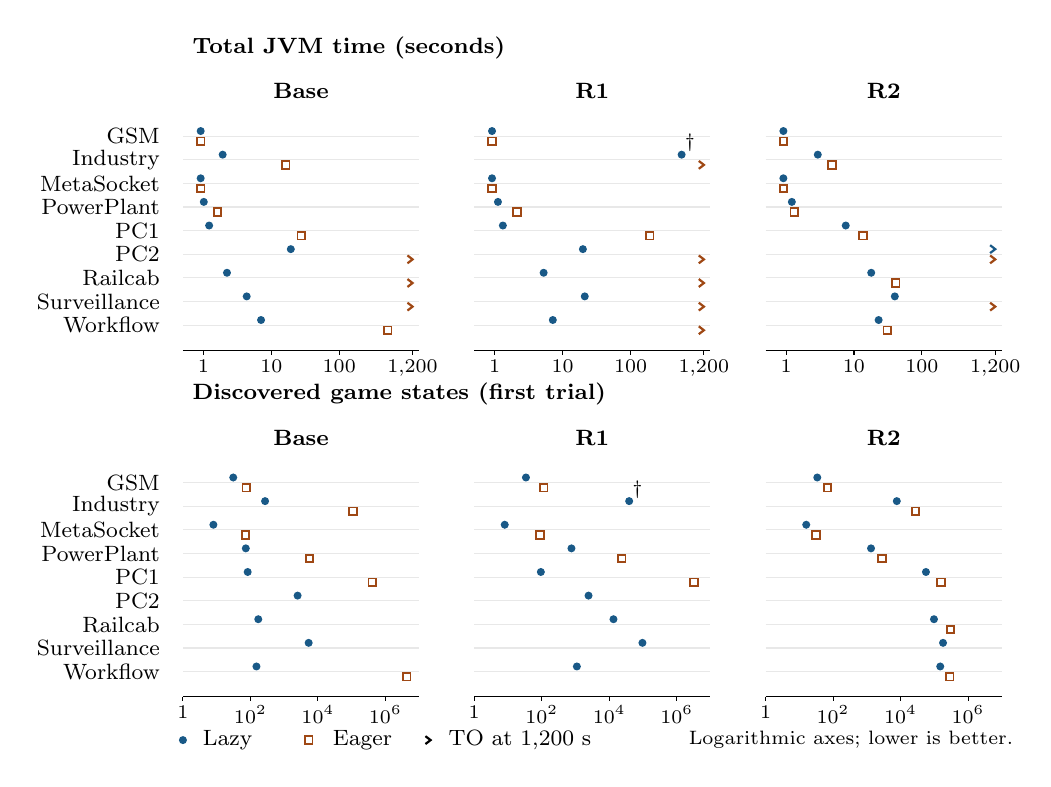
\begin{tikzpicture}[x=1cm,y=1cm,font=\footnotesize]
\definecolor{lazy}{RGB}{25,89,135}
\definecolor{eager}{RGB}{159,72,20}
\node[anchor=west,font=\footnotesize\bfseries] at (2,1.12) {Total JVM time (seconds)};
\node[font=\footnotesize\bfseries] at (3.5,0.57) {Base};
\node[anchor=east] at (1.83,0.0) {GSM};
\draw[black!9] (2.0,0.0)--(5.0,0.0);
% gsm/base/lazy: JVM median/min/max = 0.9130392/0.9125639/0.9132812
\draw[lazy,line width=.7pt] (2.22544,0.06500)--(2.22573,0.06500);
\fill[lazy] (2.22563,0.06500) circle (1.45pt);
% gsm/base/eager: JVM median/min/max = 0.9131794/0.9126908/0.9143673
\draw[eager,line width=.7pt] (2.22549,-0.06500)--(2.22618,-0.06500);
\draw[eager,fill=white,line width=.65pt] (2.17769,-0.11300) rectangle (2.27369,-0.01700);
\node[anchor=east] at (1.83,-0.3) {Industry};
\draw[black!9] (2.0,-0.3)--(5.0,-0.3);
% industry/base/lazy: JVM median/min/max = 1.9232429/1.9213733/1.9245728
\draw[lazy,line width=.7pt] (2.50442,-0.23500)--(2.50504,-0.23500);
\fill[lazy] (2.50478,-0.23500) circle (1.45pt);
% industry/base/eager: JVM median/min/max = 16.3326169/16.0183602/16.5217978
\draw[eager,line width=.7pt] (3.29905,-0.36500)--(3.31064,-0.36500);
\draw[eager,fill=white,line width=.65pt] (3.25833,-0.41300) rectangle (3.35433,-0.31700);
\node[anchor=east] at (1.83,-0.6) {MetaSocket};
\draw[black!9] (2.0,-0.6)--(5.0,-0.6);
% metasocket/base/lazy: JVM median/min/max = 0.9123447/0.8130894/0.9141439
\draw[lazy,line width=.7pt] (2.18219,-0.53500)--(2.22609,-0.53500);
\fill[lazy] (2.22535,-0.53500) circle (1.45pt);
% metasocket/base/eager: JVM median/min/max = 0.9137026/0.9102252/0.9147436
\draw[eager,line width=.7pt] (2.22448,-0.66500)--(2.22633,-0.66500);
\draw[eager,fill=white,line width=.65pt] (2.17791,-0.71300) rectangle (2.27391,-0.61700);
\node[anchor=east] at (1.83,-0.8999999999999999) {PowerPlant};
\draw[black!9] (2.0,-0.8999999999999999)--(5.0,-0.8999999999999999);
% powerplant/base/lazy: JVM median/min/max = 1.0144494/1.0141636/1.0154832
\draw[lazy,line width=.7pt] (2.26499,-0.83500)--(2.26548,-0.83500);
\fill[lazy] (2.26510,-0.83500) circle (1.45pt);
% powerplant/base/eager: JVM median/min/max = 1.618809/1.5183377/1.6203611
\draw[eager,line width=.7pt] (2.41620,-0.96500)--(2.44057,-0.96500);
\draw[eager,fill=white,line width=.65pt] (2.39221,-1.01300) rectangle (2.48821,-0.91700);
\node[anchor=east] at (1.83,-1.2) {PC1};
\draw[black!9] (2.0,-1.2)--(5.0,-1.2);
% productioncell_arms1/base/lazy: JVM median/min/max = 1.2159295/1.2146609/1.2171044
\draw[lazy,line width=.7pt] (2.33259,-1.13500)--(2.33334,-1.13500);
\fill[lazy] (2.33298,-1.13500) circle (1.45pt);
% productioncell_arms1/base/eager: JVM median/min/max = 27.6003525/27.2324243/28.5102851
\draw[eager,line width=.7pt] (3.49789,-1.26500)--(3.51507,-1.26500);
\draw[eager,fill=white,line width=.65pt] (3.45492,-1.31300) rectangle (3.55092,-1.21700);
\node[anchor=east] at (1.83,-1.5) {PC2};
\draw[black!9] (2.0,-1.5)--(5.0,-1.5);
% productioncell_arms2/base/lazy: JVM median/min/max = 19.3573477/19.1537231/19.8590448
\draw[lazy,line width=.7pt] (3.36603,-1.43500)--(3.37958,-1.43500);
\fill[lazy] (3.36999,-1.43500) circle (1.45pt);
\draw[eager,line width=.8pt] (4.85139,-1.61500)--(4.91639,-1.56500)--(4.85139,-1.51500);
\node[anchor=east] at (1.83,-1.7999999999999998) {Railcab};
\draw[black!9] (2.0,-1.7999999999999998)--(5.0,-1.7999999999999998);
% railcab/base/lazy: JVM median/min/max = 2.2257407/2.2238686/2.2280735
\draw[lazy,line width=.7pt] (2.55920,-1.73500)--(2.55991,-1.73500);
\fill[lazy] (2.55952,-1.73500) circle (1.45pt);
\draw[eager,line width=.8pt] (4.85139,-1.91500)--(4.91639,-1.86500)--(4.85139,-1.81500);
\node[anchor=east] at (1.83,-2.1) {Surveillance};
\draw[black!9] (2.0,-2.1)--(5.0,-2.1);
% surveillance/base/lazy: JVM median/min/max = 4.3426951/4.3404821/4.442846
\draw[lazy,line width=.7pt] (2.80978,-2.03500)--(2.81851,-2.03500);
\fill[lazy] (2.80997,-2.03500) circle (1.45pt);
\draw[eager,line width=.8pt] (4.85139,-2.21500)--(4.91639,-2.16500)--(4.85139,-2.11500);
\node[anchor=east] at (1.83,-2.4) {Workflow};
\draw[black!9] (2.0,-2.4)--(5.0,-2.4);
% workflow/base/lazy: JVM median/min/max = 7.0619707/6.9637387/7.0643322
\draw[lazy,line width=.7pt] (2.98691,-2.33500)--(2.99229,-2.33500);
\fill[lazy] (2.99216,-2.33500) circle (1.45pt);
% workflow/base/eager: JVM median/min/max = 518.0498148/501.4345891/528.424175
\draw[eager,line width=.7pt] (4.58942,-2.46500)--(4.60907,-2.46500);
\draw[eager,fill=white,line width=.65pt] (4.55364,-2.51300) rectangle (4.64964,-2.41700);
\draw (2.0,-2.72)--(5.0,-2.72);
\draw (2.25972,-2.72)--(2.25972,-2.7750000000000004);
\node[anchor=north,font=\scriptsize,inner sep=1pt] at (2.25972,-2.7950000000000004) {1};
\draw (3.12251,-2.72)--(3.12251,-2.7750000000000004);
\node[anchor=north,font=\scriptsize,inner sep=1pt] at (3.12251,-2.7950000000000004) {10};
\draw (3.98529,-2.72)--(3.98529,-2.7750000000000004);
\node[anchor=north,font=\scriptsize,inner sep=1pt] at (3.98529,-2.7950000000000004) {100};
\draw (4.91639,-2.72)--(4.91639,-2.7750000000000004);
\node[anchor=north,font=\scriptsize,inner sep=1pt] at (4.91639,-2.7950000000000004) {1,200};
\node[font=\footnotesize\bfseries] at (7.2,0.57) {R1};
\draw[black!9] (5.7,0.0)--(8.7,0.0);
% gsm/r1/lazy: JVM median/min/max = 0.9130627/0.9123974/0.9144691
\draw[lazy,line width=.7pt] (5.92537,0.06500)--(5.92622,0.06500);
\fill[lazy] (5.92564,0.06500) circle (1.45pt);
% gsm/r1/eager: JVM median/min/max = 0.9133292/0.9125619/0.9142938
\draw[eager,line width=.7pt] (5.92544,-0.06500)--(5.92615,-0.06500);
\draw[eager,fill=white,line width=.65pt] (5.87775,-0.11300) rectangle (5.97375,-0.01700);
\draw[black!9] (5.7,-0.3)--(8.7,-0.3);
% industry/r1/lazy: JVM median/min/max = 563.926891/536.104858/568.0240798
\draw[lazy,line width=.7pt] (8.31447,-0.23500)--(8.33614,-0.23500);
\fill[lazy] (8.33343,-0.23500) circle (1.45pt);
\node[font=\scriptsize,anchor=south west,inner sep=1pt] at (8.33343,-0.23500) {$\dagger$};
\draw[eager,line width=.8pt] (8.55139,-0.41500)--(8.61639,-0.36500)--(8.55139,-0.31500);
\draw[black!9] (5.7,-0.6)--(8.7,-0.6);
% metasocket/r1/lazy: JVM median/min/max = 0.9127905/0.9125641/0.9131296
\draw[lazy,line width=.7pt] (5.92544,-0.53500)--(5.92567,-0.53500);
\fill[lazy] (5.92553,-0.53500) circle (1.45pt);
% metasocket/r1/eager: JVM median/min/max = 0.9139618/0.9136255/0.914775
\draw[eager,line width=.7pt] (5.92587,-0.66500)--(5.92635,-0.66500);
\draw[eager,fill=white,line width=.65pt] (5.87801,-0.71300) rectangle (5.97401,-0.61700);
\draw[black!9] (5.7,-0.8999999999999999)--(8.7,-0.8999999999999999);
% powerplant/r1/lazy: JVM median/min/max = 1.1158616/1.1153371/1.1176993
\draw[lazy,line width=.7pt] (6.00062,-0.83500)--(6.00142,-0.83500);
\fill[lazy] (6.00080,-0.83500) circle (1.45pt);
% powerplant/r1/eager: JVM median/min/max = 2.1260115/2.0235737/2.1266509
\draw[eager,line width=.7pt] (6.22384,-0.96500)--(6.24245,-0.96500);
\draw[eager,fill=white,line width=.65pt] (6.19434,-1.01300) rectangle (6.29034,-0.91700);
\draw[black!9] (5.7,-1.2)--(8.7,-1.2);
% productioncell_arms1/r1/lazy: JVM median/min/max = 1.3185895/1.31351/1.3191768
\draw[lazy,line width=.7pt] (6.06191,-1.13500)--(6.06352,-1.13500);
\fill[lazy] (6.06335,-1.13500) circle (1.45pt);
% productioncell_arms1/r1/eager: JVM median/min/max = 190.9923827/187.8600834/192.6318621
\draw[eager,line width=.7pt] (7.92155,-1.26500)--(7.93095,-1.26500);
\draw[eager,fill=white,line width=.65pt] (7.87974,-1.31300) rectangle (7.97574,-1.21700);
\draw[black!9] (5.7,-1.5)--(8.7,-1.5);
% productioncell_arms2/r1/lazy: JVM median/min/max = 19.856803/19.6565302/20.2649448
\draw[lazy,line width=.7pt] (7.07574,-1.43500)--(7.08716,-1.43500);
\fill[lazy] (7.07954,-1.43500) circle (1.45pt);
\draw[eager,line width=.8pt] (8.55139,-1.61500)--(8.61639,-1.56500)--(8.55139,-1.51500);
\draw[black!9] (5.7,-1.7999999999999998)--(8.7,-1.7999999999999998);
% railcab/r1/lazy: JVM median/min/max = 5.2488108/5.24175/5.2504391
\draw[lazy,line width=.7pt] (6.58048,-1.73500)--(6.58110,-1.73500);
\fill[lazy] (6.58098,-1.73500) circle (1.45pt);
\draw[eager,line width=.8pt] (8.55139,-1.91500)--(8.61639,-1.86500)--(8.55139,-1.81500);
\draw[black!9] (5.7,-2.1)--(8.7,-2.1);
% surveillance/r1/lazy: JVM median/min/max = 21.157874/20.768775/21.266785
\draw[lazy,line width=.7pt] (7.09636,-2.03500)--(7.10524,-2.03500);
\fill[lazy] (7.10332,-2.03500) circle (1.45pt);
\draw[eager,line width=.8pt] (8.55139,-2.21500)--(8.61639,-2.16500)--(8.55139,-2.11500);
\draw[black!9] (5.7,-2.4)--(8.7,-2.4);
% workflow/r1/lazy: JVM median/min/max = 7.1662477/7.0585443/7.2598173
\draw[lazy,line width=.7pt] (6.69198,-2.33500)--(6.70252,-2.33500);
\fill[lazy] (6.69765,-2.33500) circle (1.45pt);
\draw[eager,line width=.8pt] (8.55139,-2.51500)--(8.61639,-2.46500)--(8.55139,-2.41500);
\draw (5.7,-2.72)--(8.7,-2.72);
\draw (5.95972,-2.72)--(5.95972,-2.7750000000000004);
\node[anchor=north,font=\scriptsize,inner sep=1pt] at (5.95972,-2.7950000000000004) {1};
\draw (6.82251,-2.72)--(6.82251,-2.7750000000000004);
\node[anchor=north,font=\scriptsize,inner sep=1pt] at (6.82251,-2.7950000000000004) {10};
\draw (7.68529,-2.72)--(7.68529,-2.7750000000000004);
\node[anchor=north,font=\scriptsize,inner sep=1pt] at (7.68529,-2.7950000000000004) {100};
\draw (8.61639,-2.72)--(8.61639,-2.7750000000000004);
\node[anchor=north,font=\scriptsize,inner sep=1pt] at (8.61639,-2.7950000000000004) {1,200};
\node[font=\footnotesize\bfseries] at (10.9,0.57) {R2};
\draw[black!9] (9.4,0.0)--(12.4,0.0);
% gsm/r2/lazy: JVM median/min/max = 0.9135891/0.9123249/0.9146305
\draw[lazy,line width=.7pt] (9.62534,0.06500)--(9.62629,0.06500);
\fill[lazy] (9.62586,0.06500) circle (1.45pt);
% gsm/r2/eager: JVM median/min/max = 0.9138196/0.9137006/0.9140096
\draw[eager,line width=.7pt] (9.62591,-0.06500)--(9.62603,-0.06500);
\draw[eager,fill=white,line width=.65pt] (9.57795,-0.11300) rectangle (9.67395,-0.01700);
\draw[black!9] (9.4,-0.3)--(12.4,-0.3);
% industry/r2/lazy: JVM median/min/max = 2.9308907/2.9296067/2.9327077
\draw[lazy,line width=.7pt] (10.06248,-0.23500)--(10.06287,-0.23500);
\fill[lazy] (10.06264,-0.23500) circle (1.45pt);
% industry/r2/eager: JVM median/min/max = 4.7461032/4.7437719/4.9516504
\draw[eager,line width=.7pt] (10.24307,-0.36500)--(10.25914,-0.36500);
\draw[eager,fill=white,line width=.65pt] (10.19526,-0.41300) rectangle (10.29126,-0.31700);
\draw[black!9] (9.4,-0.6)--(12.4,-0.6);
% metasocket/r2/lazy: JVM median/min/max = 0.9132551/0.9130302/0.9140156
\draw[lazy,line width=.7pt] (9.62563,-0.53500)--(9.62603,-0.53500);
\fill[lazy] (9.62572,-0.53500) circle (1.45pt);
% metasocket/r2/eager: JVM median/min/max = 0.913473/0.9128511/0.9139487
\draw[eager,line width=.7pt] (9.62556,-0.66500)--(9.62601,-0.66500);
\draw[eager,fill=white,line width=.65pt] (9.57781,-0.71300) rectangle (9.67381,-0.61700);
\draw[black!9] (9.4,-0.8999999999999999)--(12.4,-0.8999999999999999);
% powerplant/r2/lazy: JVM median/min/max = 1.2168166/1.215708/1.2173083
\draw[lazy,line width=.7pt] (9.73291,-0.83500)--(9.73341,-0.83500);
\fill[lazy] (9.73325,-0.83500) circle (1.45pt);
% powerplant/r2/eager: JVM median/min/max = 1.3178143/1.3166207/1.3182642
\draw[eager,line width=.7pt] (9.76279,-0.96500)--(9.76326,-0.96500);
\draw[eager,fill=white,line width=.65pt] (9.71513,-1.01300) rectangle (9.81113,-0.91700);
\draw[black!9] (9.4,-1.2)--(12.4,-1.2);
% productioncell_arms1/r2/lazy: JVM median/min/max = 7.5612511/7.4619858/8.2725932
\draw[lazy,line width=.7pt] (10.41281,-1.13500)--(10.45145,-1.13500);
\fill[lazy] (10.41776,-1.13500) circle (1.45pt);
% productioncell_arms1/r2/eager: JVM median/min/max = 13.611786/13.5977826/14.1108414
\draw[eager,line width=.7pt] (10.63766,-1.26500)--(10.65154,-1.26500);
\draw[eager,fill=white,line width=.65pt] (10.59005,-1.31300) rectangle (10.68605,-1.21700);
\draw[black!9] (9.4,-1.5)--(12.4,-1.5);
\draw[lazy,line width=.8pt] (12.25139,-1.48500)--(12.31639,-1.43500)--(12.25139,-1.38500);
\draw[eager,line width=.8pt] (12.25139,-1.61500)--(12.31639,-1.56500)--(12.25139,-1.51500);
\draw[black!9] (9.4,-1.7999999999999998)--(12.4,-1.7999999999999998);
% railcab/r2/lazy: JVM median/min/max = 17.933768/17.8337679/17.9398622
\draw[lazy,line width=.7pt] (10.73927,-1.73500)--(10.74150,-1.73500);
\fill[lazy] (10.74137,-1.73500) circle (1.45pt);
% railcab/r2/eager: JVM median/min/max = 41.1987655/41.1810933/41.3951525
\draw[eager,line width=.7pt] (11.05286,-1.86500)--(11.05480,-1.86500);
\draw[eager,fill=white,line width=.65pt] (11.00502,-1.91300) rectangle (11.10102,-1.81700);
\draw[black!9] (9.4,-2.1)--(12.4,-2.1);
% surveillance/r2/lazy: JVM median/min/max = 39.8928114/39.8765955/40.3825681
\draw[lazy,line width=.7pt] (11.04080,-2.03500)--(11.04552,-2.03500);
\fill[lazy] (11.04095,-2.03500) circle (1.45pt);
\draw[eager,line width=.8pt] (12.25139,-2.21500)--(12.31639,-2.16500)--(12.25139,-2.11500);
\draw[black!9] (9.4,-2.4)--(12.4,-2.4);
% workflow/r2/lazy: JVM median/min/max = 23.0530876/22.7744215/23.3715254
\draw[lazy,line width=.7pt] (10.83091,-2.33500)--(10.84060,-2.33500);
\fill[lazy] (10.83546,-2.33500) circle (1.45pt);
% workflow/r2/eager: JVM median/min/max = 30.9360675/30.4163997/31.6364434
\draw[eager,line width=.7pt] (10.93932,-2.46500)--(10.95406,-2.46500);
\draw[eager,fill=white,line width=.65pt] (10.89767,-2.51300) rectangle (10.99367,-2.41700);
\draw (9.4,-2.72)--(12.4,-2.72);
\draw (9.65972,-2.72)--(9.65972,-2.7750000000000004);
\node[anchor=north,font=\scriptsize,inner sep=1pt] at (9.65972,-2.7950000000000004) {1};
\draw (10.52251,-2.72)--(10.52251,-2.7750000000000004);
\node[anchor=north,font=\scriptsize,inner sep=1pt] at (10.52251,-2.7950000000000004) {10};
\draw (11.38529,-2.72)--(11.38529,-2.7750000000000004);
\node[anchor=north,font=\scriptsize,inner sep=1pt] at (11.38529,-2.7950000000000004) {100};
\draw (12.31639,-2.72)--(12.31639,-2.7750000000000004);
\node[anchor=north,font=\scriptsize,inner sep=1pt] at (12.31639,-2.7950000000000004) {1,200};
\node[anchor=west,font=\footnotesize\bfseries] at (2,-3.2800000000000002) {Discovered game states (first trial)};
\node[font=\footnotesize\bfseries] at (3.5,-3.8300000000000005) {Base};
\node[anchor=east] at (1.83,-4.4) {GSM};
\draw[black!9] (2.0,-4.4)--(5.0,-4.4);
% gsm/base/lazy: first-trial states = 31
\fill[lazy] (2.63916,-4.33500) circle (1.45pt);
% gsm/base/eager: first-trial states = 75
\draw[eager,fill=white,line width=.65pt] (2.75560,-4.51300) rectangle (2.85160,-4.41700);
\node[anchor=east] at (1.83,-4.7) {Industry};
\draw[black!9] (2.0,-4.7)--(5.0,-4.7);
% industry/base/lazy: first-trial states = 272
\fill[lazy] (3.04339,-4.63500) circle (1.45pt);
% industry/base/eager: first-trial states = 109726
\draw[eager,fill=white,line width=.65pt] (4.11213,-4.81300) rectangle (4.20813,-4.71700);
\node[anchor=east] at (1.83,-5.0) {MetaSocket};
\draw[black!9] (2.0,-5.0)--(5.0,-5.0);
% metasocket/base/lazy: first-trial states = 8
\fill[lazy] (2.38704,-4.93500) circle (1.45pt);
% metasocket/base/eager: first-trial states = 71
\draw[eager,fill=white,line width=.65pt] (2.74540,-5.11300) rectangle (2.84140,-5.01700);
\node[anchor=east] at (1.83,-5.300000000000001) {PowerPlant};
\draw[black!9] (2.0,-5.300000000000001)--(5.0,-5.300000000000001);
% powerplant/base/lazy: first-trial states = 73
\fill[lazy] (2.79857,-5.23500) circle (1.45pt);
% powerplant/base/eager: first-trial states = 5634
\draw[eager,fill=white,line width=.65pt] (3.55949,-5.41300) rectangle (3.65549,-5.31700);
\node[anchor=east] at (1.83,-5.6000000000000005) {PC1};
\draw[black!9] (2.0,-5.6000000000000005)--(5.0,-5.6000000000000005);
% productioncell_arms1/base/lazy: first-trial states = 83
\fill[lazy] (2.82246,-5.53500) circle (1.45pt);
% productioncell_arms1/base/eager: first-trial states = 407019
\draw[eager,fill=white,line width=.65pt] (4.35612,-5.71300) rectangle (4.45212,-5.61700);
\node[anchor=east] at (1.83,-5.9) {PC2};
\draw[black!9] (2.0,-5.9)--(5.0,-5.9);
% productioncell_arms2/base/lazy: first-trial states = 2502
\fill[lazy] (3.45641,-5.83500) circle (1.45pt);
\node[anchor=east] at (1.83,-6.2) {Railcab};
\draw[black!9] (2.0,-6.2)--(5.0,-6.2);
% railcab/base/lazy: first-trial states = 171
\fill[lazy] (2.95700,-6.13500) circle (1.45pt);
\node[anchor=east] at (1.83,-6.5) {Surveillance};
\draw[black!9] (2.0,-6.5)--(5.0,-6.5);
% surveillance/base/lazy: first-trial states = 5319
\fill[lazy] (3.59678,-6.43500) circle (1.45pt);
\node[anchor=east] at (1.83,-6.800000000000001) {Workflow};
\draw[black!9] (2.0,-6.800000000000001)--(5.0,-6.800000000000001);
% workflow/base/lazy: first-trial states = 151
\fill[lazy] (2.93385,-6.73500) circle (1.45pt);
% workflow/base/eager: first-trial states = 4292588
\draw[eager,fill=white,line width=.65pt] (4.79459,-6.91300) rectangle (4.89059,-6.81700);
\draw (2.0,-7.120000000000001)--(5.0,-7.120000000000001);
\draw (2.00000,-7.120000000000001)--(2.00000,-7.175000000000001);
\node[anchor=north,font=\scriptsize,inner sep=1pt] at (2.00000,-7.195000000000001) {1};
\draw (2.85714,-7.120000000000001)--(2.85714,-7.175000000000001);
\node[anchor=north,font=\scriptsize,inner sep=1pt] at (2.85714,-7.195000000000001) {$10^2$};
\draw (3.71429,-7.120000000000001)--(3.71429,-7.175000000000001);
\node[anchor=north,font=\scriptsize,inner sep=1pt] at (3.71429,-7.195000000000001) {$10^4$};
\draw (4.57143,-7.120000000000001)--(4.57143,-7.175000000000001);
\node[anchor=north,font=\scriptsize,inner sep=1pt] at (4.57143,-7.195000000000001) {$10^6$};
\node[font=\footnotesize\bfseries] at (7.2,-3.8300000000000005) {R1};
\draw[black!9] (5.7,-4.4)--(8.7,-4.4);
% gsm/r1/lazy: first-trial states = 34
\fill[lazy] (6.35635,-4.33500) circle (1.45pt);
% gsm/r1/eager: first-trial states = 114
\draw[eager,fill=white,line width=.65pt] (6.53353,-4.51300) rectangle (6.62953,-4.41700);
\draw[black!9] (5.7,-4.7)--(8.7,-4.7);
% industry/r1/lazy: first-trial states = 38942
\fill[lazy] (7.66732,-4.63500) circle (1.45pt);
\node[font=\scriptsize,anchor=south west,inner sep=1pt] at (7.66732,-4.63500) {$\dagger$};
\draw[black!9] (5.7,-5.0)--(8.7,-5.0);
% metasocket/r1/lazy: first-trial states = 8
\fill[lazy] (6.08704,-4.93500) circle (1.45pt);
% metasocket/r1/eager: first-trial states = 88
\draw[eager,fill=white,line width=.65pt] (6.48535,-5.11300) rectangle (6.58135,-5.01700);
\draw[black!9] (5.7,-5.300000000000001)--(8.7,-5.300000000000001);
% powerplant/r1/lazy: first-trial states = 759
\fill[lazy] (6.93439,-5.23500) circle (1.45pt);
% powerplant/r1/eager: first-trial states = 23352
\draw[eager,fill=white,line width=.65pt] (7.52414,-5.41300) rectangle (7.62014,-5.31700);
\draw[black!9] (5.7,-5.6000000000000005)--(8.7,-5.6000000000000005);
% productioncell_arms1/r1/lazy: first-trial states = 94
\fill[lazy] (6.54563,-5.53500) circle (1.45pt);
% productioncell_arms1/r1/eager: first-trial states = 3252233
\draw[eager,fill=white,line width=.65pt] (8.44293,-5.71300) rectangle (8.53893,-5.61700);
\draw[black!9] (5.7,-5.9)--(8.7,-5.9);
% productioncell_arms2/r1/lazy: first-trial states = 2433
\fill[lazy] (7.15120,-5.83500) circle (1.45pt);
\draw[black!9] (5.7,-6.2)--(8.7,-6.2);
% railcab/r1/lazy: first-trial states = 13339
\fill[lazy] (7.46791,-6.13500) circle (1.45pt);
\draw[black!9] (5.7,-6.5)--(8.7,-6.5);
% surveillance/r1/lazy: first-trial states = 96301
\fill[lazy] (7.83584,-6.43500) circle (1.45pt);
\draw[black!9] (5.7,-6.800000000000001)--(8.7,-6.800000000000001);
% workflow/r1/lazy: first-trial states = 1098
\fill[lazy] (7.00312,-6.73500) circle (1.45pt);
\draw (5.7,-7.120000000000001)--(8.7,-7.120000000000001);
\draw (5.70000,-7.120000000000001)--(5.70000,-7.175000000000001);
\node[anchor=north,font=\scriptsize,inner sep=1pt] at (5.70000,-7.195000000000001) {1};
\draw (6.55714,-7.120000000000001)--(6.55714,-7.175000000000001);
\node[anchor=north,font=\scriptsize,inner sep=1pt] at (6.55714,-7.195000000000001) {$10^2$};
\draw (7.41429,-7.120000000000001)--(7.41429,-7.175000000000001);
\node[anchor=north,font=\scriptsize,inner sep=1pt] at (7.41429,-7.195000000000001) {$10^4$};
\draw (8.27143,-7.120000000000001)--(8.27143,-7.175000000000001);
\node[anchor=north,font=\scriptsize,inner sep=1pt] at (8.27143,-7.195000000000001) {$10^6$};
\node[font=\footnotesize\bfseries] at (10.9,-3.8300000000000005) {R2};
\draw[black!9] (9.4,-4.4)--(12.4,-4.4);
% gsm/r2/lazy: first-trial states = 34
\fill[lazy] (10.05635,-4.33500) circle (1.45pt);
% gsm/r2/eager: first-trial states = 68
\draw[eager,fill=white,line width=.65pt] (10.13736,-4.51300) rectangle (10.23336,-4.41700);
\draw[black!9] (9.4,-4.7)--(12.4,-4.7);
% industry/r2/lazy: first-trial states = 7717
\fill[lazy] (11.06605,-4.63500) circle (1.45pt);
% industry/r2/eager: first-trial states = 27752
\draw[eager,fill=white,line width=.65pt] (11.25627,-4.81300) rectangle (11.35227,-4.71700);
\draw[black!9] (9.4,-5.0)--(12.4,-5.0);
% metasocket/r2/lazy: first-trial states = 16
\fill[lazy] (9.91605,-4.93500) circle (1.45pt);
% metasocket/r2/eager: first-trial states = 31
\draw[eager,fill=white,line width=.65pt] (9.99116,-5.11300) rectangle (10.08716,-5.01700);
\draw[black!9] (9.4,-5.300000000000001)--(12.4,-5.300000000000001);
% powerplant/r2/lazy: first-trial states = 1330
\fill[lazy] (10.73879,-5.23500) circle (1.45pt);
% powerplant/r2/eager: first-trial states = 2810
\draw[eager,fill=white,line width=.65pt] (10.83002,-5.41300) rectangle (10.92602,-5.31700);
\draw[black!9] (9.4,-5.6000000000000005)--(12.4,-5.6000000000000005);
% productioncell_arms1/r2/lazy: first-trial states = 56443
\fill[lazy] (11.43640,-5.53500) circle (1.45pt);
% productioncell_arms1/r2/eager: first-trial states = 158218
\draw[eager,fill=white,line width=.65pt] (11.58025,-5.71300) rectangle (11.67625,-5.61700);
\draw[black!9] (9.4,-5.9)--(12.4,-5.9);
\draw[black!9] (9.4,-6.2)--(12.4,-6.2);
% railcab/r2/lazy: first-trial states = 97522
\fill[lazy] (11.53819,-6.13500) circle (1.45pt);
% railcab/r2/eager: first-trial states = 299700
\draw[eager,fill=white,line width=.65pt] (11.69915,-6.31300) rectangle (11.79515,-6.21700);
\draw[black!9] (9.4,-6.5)--(12.4,-6.5);
% surveillance/r2/lazy: first-trial states = 181116
\fill[lazy] (11.65341,-6.43500) circle (1.45pt);
\draw[black!9] (9.4,-6.800000000000001)--(12.4,-6.800000000000001);
% workflow/r2/lazy: first-trial states = 149647
\fill[lazy] (11.61789,-6.73500) circle (1.45pt);
% workflow/r2/eager: first-trial states = 285348
\draw[eager,fill=white,line width=.65pt] (11.69002,-6.91300) rectangle (11.78602,-6.81700);
\draw (9.4,-7.120000000000001)--(12.4,-7.120000000000001);
\draw (9.40000,-7.120000000000001)--(9.40000,-7.175000000000001);
\node[anchor=north,font=\scriptsize,inner sep=1pt] at (9.40000,-7.195000000000001) {1};
\draw (10.25714,-7.120000000000001)--(10.25714,-7.175000000000001);
\node[anchor=north,font=\scriptsize,inner sep=1pt] at (10.25714,-7.195000000000001) {$10^2$};
\draw (11.11429,-7.120000000000001)--(11.11429,-7.175000000000001);
\node[anchor=north,font=\scriptsize,inner sep=1pt] at (11.11429,-7.195000000000001) {$10^4$};
\draw (11.97143,-7.120000000000001)--(11.97143,-7.175000000000001);
\node[anchor=north,font=\scriptsize,inner sep=1pt] at (11.97143,-7.195000000000001) {$10^6$};
\fill[lazy] (2,-7.67) circle (1.45pt);
\node[anchor=west] at (2.13,-7.67) {Lazy};
\draw[eager,fill=white,line width=.65pt] (3.55,-7.718) rectangle (3.646,-7.622);
\node[anchor=west] at (3.78,-7.67) {Eager};
\draw[black,line width=.8pt] (5.08,-7.72)--(5.145,-7.67)--(5.08,-7.62);
\node[anchor=west] at (5.25,-7.67) {TO at 1,200 s};
\node[anchor=west,font=\scriptsize] at (8.3,-7.67) {Logarithmic axes; lower is better.};
\end{tikzpicture}
\caption{All 27 contracts under the same UC pruning. Completed times are five-run medians with min--max bars, including preparation, solving, checking and other JVM work. TO arrows mark one capped attempt, not a median or a solver-time bound; no state count is imputed. $\dagger$ is Industry/R1 LOSS; other completed points are WIN.}
\label{fig:rq3-paired-absolute}
\Description{Three columns show Base, R1 and R2 for all nine adapted inputs. Upper panels show complete JVM time, lower panels show first-trial discovered states. Lazy decides 26 contracts including Industry R1 LOSS; Eager decides 17. Their 17 common completions have both markers; nine contracts have only a Lazy completion; PC2 R2 times out with both. All 11 timeouts have capped-attempt arrows in the time panels and no imputed state markers.}
\end{figure}


Lazy's adapter medians reach 14.221~s (PC2/R1; S4). Capped Direct-Full JVM totals are lower bounds, not solver medians or ratios. Auxiliary Full+UC timings mix builds, hosts and repeats, preventing pruning isolation; unpruned OTF is unimplemented (Technical Appendix~\ref{ta:performance_scope_details}).

% FGDUCS_RELOCATED: workload_rows

\paragraph{Scaling limits.}\label{sec:rq4}
The independent family exhibits the expected benefit of lazy construction under the default order; S4 gives every size and method.

Travel reaches timeouts and out-of-memory failures under all methods, including expanded-budget timeouts. These separate trials never enter medians; Technical Appendix~\ref{ta:performance_scope_details} retains all populations and adverse outcomes.

\Needspace{4\baselineskip}
\section{Related Work}
\label{sec:related}
\label{sec:expressiveness}
\paragraph{Generating update environments.}
Yamauchi et al. generate an update environment from pre/post environments and supplied global state-preservation transitions~\cite[Sec.~V]{Yamauchi2020Partitioning}. DUCS adds \texttt{reconfigure} edges through $R$ without a UC-quiescence guard; a partial $R$ can restrict its source states~\cite[Sec.~4.2, Defs.~3.7, 5.1]{Nahabedian2020}. FG gates every command and handover on global UC quiescence.

\paragraph{On-demand synthesis.}
DCS already uses on-demand component products, defers controllable alternatives, treats UC-enabled states as uncontrollable and propagates success/failure backward~\cite[Sec.~IV]{CiolekDCS}. Its 2016 formulation requires safety and eventual goal occurrence on every trace; OTF-DCS (2023) requires a marked extension of each finite controlled trace~\cite[Def.~4]{CiolekEtAl2023OTFDCS}. FG specializes these patterns to its generated contract, with complete outcome buckets and all-entry certificates. Compositional and modular approaches structure control specifications~\cite{MohajeraniMalikFabian2014Compositional,WonhamRamadge1988Modular}.

\paragraph{Supervisor switching.}
Reinitializing supervisor state can provide safe, deadlock-free switching on one plant~\cite[Sec.~3.3]{MeiraGoesLafortune2020Switching}. Workcell reconfiguration~\cite{JiaoGanXiao2013Reconfiguration}, bounded startup~\cite{NooruldeenSchmidt2015} and switched-system invariants~\cite{ReveliotisFei2017SwitchedDES} address related switching conditions. S5 compares their assumptions with FG-DUCS's staged transfers and fixed endpoint.

\paragraph{Requirements across adaptation.}
Temporal adaptation~\cite{ZhangCheng2006ALTL}, scenario-based updatability~\cite{Ghezzi2012DynamicScenarioUpdate,PanzicaLaManna2013CorrectnessDynamicUpdates} and Live Synthesis~\cite{FinkbeinerEtAl2022LiveSynthesis} address obligations across change. Our initialization uses scoped requirements~\cite{Dwyer1999Patterns} and residual reasoning~\cite{RosuHavelund2005Rewriting}. Thuijsman and Reniers~\cite[Secs.~4--7]{ThuijsmanReniers2024DynamicFeature} allow individual or simultaneous reconfiguration, requirements that depend on features, and state retention or reset. Their supervisor permits a marked continuation from every reachable state; FG requires every maximal update run to finish at a supplied controller.

\paragraph{Adaptation and operational updates.}
Safe adaptation graphs support minimum-cost paths~\cite{Zhang2005SafeAdaptation}; architectural reconfiguration sequences preserve lifecycle and architecture constraints, including consistent recovery states~\cite{BoyerGruberPous2013}. Local updating, PROTEOS, workflow updating, Kitsune and network synthesis address migration and transition safety~\cite{PanzicaLaManna2012LocalUpdate,Giuffrida2013SafeLiveUpdate,Sokolowski2022DynamicWorkflowUpdates,e6_hayden2014_kitsune,McClurgEtAl2015NetworkUpdates}. Version-consistent updating uses dynamic dependencies and selective blocking~\cite{MaEtAl2011VersionConsistency}. FG-DUCS addresses a different guarantee: finite handover under declared requirement lifetimes. It provides neither cost optimization, repair nor transaction-version consistency. S5 gives the detailed comparison.

\section{Threats to Validity}
\label{sec:threats}
\paragraph{Model and execution.}
Perpetual arrivals or polling can preclude quiescence. Waiting that relies on fairness is outside the model. The effects of adapting inherited inputs have not been isolated. Actual decoding, history completeness and A1--A4 remain unvalidated; repair is excluded.

\paragraph{Evaluation coverage.}
Constructed cases assume finite startup, reporting, recovery and election and may favor separations. They establish mechanisms, not deployed prevalence. Inherited inputs omit precedence and have branching transfers only in Railcab; fixtures and repeats are not independent applications. Null/LOSS results, faster Update-first cases, lower Eager/Update-first memory and Travel/PC failures bound the gains. PC2's merged timeout remains unresolved.

\paragraph{Implementation and measurement.}
Shared authorship, AI and code risk correlated faults; independent parsing covers restricted FSP. Direct-Full is internal and Legacy solves a different objective. External solvers, randomized orders and isolated pruning remain untested. Timing uses one machine, ratios omit unresolved costs, and extended trials lack medians. RSS sampling may miss peaks and identifies neither heap occupancy nor bottlenecks. S4 retains interruptions. The exponential separation depends on the default order.

\section{Conclusion}
\label{sec:conclusion}
FG-DUCS compiles local transfers, requirement lifetimes and initializers into safe finite updates preserving the selected endpoint's continuation. Merging commands can help or prevent completion. With the same UC pruning, Lazy decides \FixedLazyDecisions{}/\ApplicationContracts{} contracts to Eager's \FixedEagerDecisions{}; Update-first is sometimes faster. Guarantees require declared lifetimes, UC quiescence and faithful execution.

\clearpage
\section*{Data Availability}
We created and publicly released the anonymous FG-DUCS replication package for this paper~\cite{FGDUCSAnonymousArtifact}. The retained evidence snapshot is available at \url{https://github.com/research-artifact-archive/research-artifact/tree/fgducs-invariants-20261002}. The paper-matched release cited in~\cite{FGDUCSAnonymousArtifact}, \texttt{fgducs-c105-20261003}, contains this revised main paper and \texttt{paper/supplementary\_material.pdf}: Part I is Technical Appendix A--P; Part II is Supplement S1--S5. Its reading guide, bookmarks and continuous page numbers locate the proofs, full models and experimental records cited throughout the main text. The repository README links directly to both parts and maps paper sections to evidence. The package also provides source code, all 27 application contracts, scripts and saved results; saved-evidence checks require no new performance experiments. Dependencies come from official upstream sources.

\bibliographystyle{ACM-Reference-Format}
\bibliography{references}

\end{document}
